\documentclass[a4paper,11pt,oneside]{article}%pridat twoside, do [] pre obojstrannu tlac
    \pagestyle{headings}
    %\linespread{1.15} % riadkovanie
    \usepackage[top=2.5cm, bottom=2.5cm, left=3.5cm, right=2cm]{geometry} %odporucane okraje
%    \usepackage[top=2.9cm, bottom=2.9cm, left=2.5cm, right=4cm]{geometry} %okraje
    %\evensidemargin=-0cm       %uprava okrajov
    %\oddsidemargin=+1.5cm        %uprava okrajov

%Slovencina
\usepackage[slovak]{babel}
\usepackage[utf8x]{inputenc}
%\usepackage[cp1250]{inputenc}
\usepackage[T1]{fontenc} %pekne makcene


%male popisy obrazkov a~grafika
\usepackage[font=small,margin=0.5cm]{caption} % margin reguluje okraje popisu obrazka (v pripade, ze je na sirku strany a~ma viac ako 1 riadok)
%\usepackage[dvips]{graphicx}
\usepackage{wrapfig}
%\usepackage[pdftex]{graphicx}
\usepackage[usenames,dvipsnames]{color}
\usepackage{epstopdf}   %bez tohto pdflatex nezoberie eps obazky

\usepackage{float} %kvoli H pri oberazkoch

\usepackage{graphicx}
%\usepackage{url}
%\usepackage[hidelinks, breaklinks]{hyperref}
%\usepackage{float}

%grid obrazkov
\usepackage{subfig}

%farebne tabulky
\usepackage{colortbl}
%\usepackage[table]{xcolor}
%na otacanie tabuliek
\usepackage{rotating}

%odsadenie prveho odstavca
\usepackage{indentfirst}

%Matematicke vyrazy
\usepackage{amsfonts}
\usepackage{amsmath}
\usepackage{amssymb}

\usepackage{verbatim}
\usepackage[official]{eurosym}
\usepackage{url}

%algoritmy
\usepackage[lined,boxed]{algorithm2e}

%�moje definicie
\newcommand{\p}{\partial}
 \def\epsilon{\varepsilon}
 \def\Bf#1{\mathbf{#1}}
 
 \makeatletter
\newsavebox\myboxA
\newsavebox\myboxB
\newlength\mylenA

\newcommand*\xoverline[2][0.75]{%
    \sbox{\myboxA}{$\m@th#2$}%
    \setbox\myboxB\null% Phantom box
    \ht\myboxB=\ht\myboxA%
    \dp\myboxB=\dp\myboxA%
    \wd\myboxB=#1\wd\myboxA% Scale phantom
    \sbox\myboxB{$\m@th\overline{\copy\myboxB}$}%  Overlined phantom
    \setlength\mylenA{\the\wd\myboxA}%   calc width diff
    \addtolength\mylenA{-\the\wd\myboxB}%
    \ifdim\wd\myboxB<\wd\myboxA%
       \rlap{\hskip 0.5\mylenA\usebox\myboxB}{\usebox\myboxA}%
    \else
        \hskip -0.5\mylenA\rlap{\usebox\myboxA}{\hskip 0.5\mylenA\usebox\myboxB}%
    \fi}
\makeatother

%Slovenske uvodzovky
\chardef\clqq=18 \sfcode18=0
\chardef\crqq=16 \sfcode16=0
\def\uv#1{\clqq#1\crqq}

\usepackage{verse}

\author{Mária Somorovská}
\title{Automatické segmentačné metódy biologických dát}

%Hyperreferencia
\usepackage{hyperref}
    \hypersetup{colorlinks,citecolor=red,filecolor=black,linkcolor=blue,urlcolor=blue,pdftex}
%====================================================================================================================================================
%====================================================================================================================================================

\begin{document}
\setlength{\belowdisplayskip}{7pt} \setlength{\belowdisplayshortskip}{5pt}
\setlength{\abovedisplayskip}{7pt} \setlength{\abovedisplayshortskip}{5pt}

%***********************zaciatok prvej strany
    \thispagestyle{empty}
    {
    \topmargin=0pt
    \centerline {\large \bf{SLOVENSKÁ TECHNICKÁ UNIVERZITA V~BRATISLAVE}}
    \vskip 0.2cm
    \centerline{\large \bf{STAVEBNÁ FAKULTA}}
    \vskip 7cm
    \centerline{\Large \bf{Automatické segmentačné metódy biologických dát}}
    \vskip 0.2cm
    %\centerline{\Large \bf{V PRÍPADE, ŽE JE PRIDLHÝ JEHO DRUHÝ RIADOK}}
    %\centerline{ \bf{(verzia z~\today) }}   %vypisovanie dnesneho datumu
    \vskip 0.5cm
    \centerline{\large \bf{Diplomová práca}}
    \vskip 5cm          %\vskip 2cm             %zmena kvoli zobrazovaniu dnesneho datumu
    \normalsize
        \begin{tabular}[l]{p{0.27\textwidth}p{0.73\textwidth}}
        Študijny program: & Matematicko-počítačové modelovanie\\
        Študijny odbor: & Aplikovaná matematika\\
        Školiace pracovisko: & Katedra matematiky a deskriptívnej geometrie\\
        Vedúci diplomovej\\ práce: & doc. RNDr. Zuzana Krivá, PhD. \\
        \end{tabular}
    \vskip 1.5cm
    \centerline{\large \bf{BRATISLAVA 2020}}
    \vskip 0.2cm
    \centerline{\large \bf{Bc. Mária Somorovská}}
    }
\pagebreak
%**********************************koniec prvej strany

%obsah
\tableofcontents

\newpage

\section{Úvod}
% In the different 
%Spracovanie obrazov, je metóda, ktorá používa rôzne operácie na obrazových dátach

%Makrofág je typ pohyblivej bielej krvinky, ktorá hrá dôležitú úlohu v ochrane imunitného systému  

%Dáta, ktorými sa zaoberá táto 
%Rôzne vedné odvetvia, využivajú

V rôznych vedných disciplínach ale aj v bežnom živote sa používajú rôzne aplikácie spracovania obrazov. Spracovanie obrazov je metóda, ktorá pomocou rôznych matematických operácii a algoritmov upravuje obrazové dáta rôznych formátov a pomáha z nich získavať užitočné informácie. Obrazové dáta je potrebné zobraziť, či už pred alebo po modifikácií. 

Cieľom práce je vytvorenie softvéru, ktorý slúži na vizualizáciu a segmentáciu obrazov získaných konfokálnym laserovým mikroskopom, konkrétne sa jedná o biologické dáta a to obrazy makrofágov. Takéto dáta môžu obsahovať šum, ktorý je potrebné odstrániť pre lepšie rozoznanie objektov na dátach. 
 
Z biologického hľadiska, je maktofág typ bielej krvinky, ktorá hrá dôležitú úlohu pri ochrane imunitného systému a hemostázy. Avšak disfunkčné makrofágy menia svoje účinky a u ľudí môžu spôsobovať závažné ochorenia ako sú napríklad  zápalové ochorenia, ktoré vedú k častým infekciám alebo sa môžu podieľať na postupe rakoviny. Makrofág mení svoj tvar keď sa približuje smerom k rane. Táto zmena tvaru je spôsobená objektami, ktoré sa nachádzajú v blízkosti makrofágu, ako napríklad tkanivovými bunkami alebo medzibunkovou hmotou.
Segmentácia obrazov môže byť užitočným nástrojom na porozumenie spôsobu interakcie medzi makrofágmi a bunkami, ktoré ho obklopujú, avšak takáto segmentácia môže byť náročnou úlohou, kvôli ich nepravidelnému tvaru.

Mikroskopové dáta makrofágov, s ktorými pracujeme v tejto práci, sú makrofágy priesvitného embrya zebričky pruhovanej (\textit{lat.} danio rerio). Táto larva bola poranená a cytoplazmy makrofágov sú zafarbené zeleným svetielkujúcim proteínom (kaede) pre lepšiu viditeľnosť pod mikroskopom. Pôvodné dáta makrofágov sú získané v časovom úseku 5 hodín a s časovým krokom 4 minúty. Následne dané trojdimenzionálne obrazové dáta sú premietnuté do roviny za použitia maximálnej intenzity približne zo 70 rezov, z ktorých vzniknú dvoj-dimenzionálne obrazové dáta. 
%vo formáte tiff.

V tejto práci sa zaoberáme časťami/výrezmi takýchto dát, na ktorých sa nachádza jeden makrofág a používame rôzne metódy na segmentáciu, buď automatické alebo semi-automatické. Softvér by mal byť intuitívny, a teda určený aj užívateľom, ktorí implementovaným algoritmom nemusia rozumieť. 
  
Práca je rozdelená do viacerých častí, v ktorých je podrobnejšie popísaná funkcionalita programu spolu s užívateľským prostredím, použitými algoritmami, knižnicami.

Prvá časť je teoretická a venuje sa matematickým algoritmom využitých pri implementácii, založených na poznatkoch zo spracovania obrazov. Jedná sa o niekoľko automatických a semi-automatických segmentačných metód, ktoré sú kombináciou prahovacích metód a segmentačnej metódy subjektívnych plôch(SUBSURF).

Druhá časť sa zameriava na technológie a knižnice využité pri implementácii. Nachádza sa tam popis Qt knižníc, ktoré boli použité pri vytváraní užívateľského prostredia, VTK knižníc, ktoré boli využité na zobrazenie a manipuláciu s dátami. Popísané sú tu aj triedy, ktoré boli v programe najviac využité.

Ďaľšia časť sa zaoberá popisom grafického rozhrania programu, ktorá by mohla slúžiť aj ako manuál slúžiaci užívateľovi pri používaní.

V poslednej časti sa nachádzajú výsledky, ku ktorým sme v práci dospeli a porovnania medzi rôznymi automatickými a semi-automatickými segmentačnými metódami.

% užité matematické algoritmy, funkcionalita naimplementovaného softvéru a 
  
 
%Skúmané dáta pochadzajú pôvodne z  a sú z

\newpage

\section{Segmentácie obrazov} \label{math}

%

Hlavnou úlohou pri segmentácii makrofágov, je rozlíšenie pozadia a objektu na obrazových dátach. Táto úloha môže byť sťažená kvôli strate intenzity na hranách alebo šumu, ktorý sa môže na dátach nachádzať.

%Hlavnou úlohou pri segmentácii makrofágov je odstránenie šumu, ktorý môže byť spôsobený premietnutím dát z trojdimenzionálneho priestoru do roviny alebo bunkami nachádzajúcimi sa v okolí makrofágu alebo zmenou tvaru v čase.

Segmentácia takýchto dát je náročnou úlohou pretože makrofágy majú nepravidelné tvary s meniacou sa intenzitou, ktoré sa ťažko spracovávajú. Preto sme vybrali niekoľko druhov prahovacích metód, ktoré sme skombinovali spolu s metódou segmentácie subjektívnych plôch a aplikovali sme ich na testované dáta.

\subsection{Globálne prahovanie}

 Úlohou globálnych prahovacích metód je nájsť jedinú optimálnu prahovú hodnotu $q$, v našom prípade šedo-tónových obrazových dát, ktorá zadefinuje každý pixel obrazu buď do popredia (ako objekt na dátach) alebo ako pozadie. Mnohé z týchto metód sú založené na histograme. Teda všetky pixely sú zatriedené do dvoch disjunktných množín $C_0$ a $C_1$, kde množina $C_0$ obsahuje všetky pixle nachádzajúce sa medzi hodnotami $(0, 1, \dots , q)$ a $C_1$ obsahuje všetky zvyšné pixle nachádzajúce sa na intervale $(q+1, \dots , K-1)$, teda

\begin{equation}
(u, v) \in \begin{cases} C_0 & \text{ak} \hspace{1em} I(u,v) \leq q \hspace{1em} \text{(pozadie)} \\  C_1 & \text{ak} \hspace{1em} I(u,v) \geq q \hspace{1em} \text{(objekt)} \end{cases}.
\end{equation}

%preformulovat
Treba si uvedomiť, že tieto hodnoty závisia od toho, či je pozadie bledé a objekt tmavý alebo naopak.

Prahovacie metódy založené na histograme sú zvyčajne jednoduché a účinné, pretože pracujú s malým množstvom dát. V našom prípade sa jedná o 256 odtieňov sivej/šede. Dajú sa rozdeliť na 2 hlavné kategórie: štatistické metódy a také, ktoré sú založené na tvare.


\subsubsection{Otsuho metóda} \label{OtsuM}
Otsuho metóda\cite{otsu} patrí medzi automatické  prahovacie metódy, ktorá rozdeľuje obrazové dáta na 2 rôzne triedy pomocou prahu $q$ $-$ na objekt a pozadie. Hlavnou myšlienkou tejto metódy je nájsť prah $q$ taký, že výsledné distribúcie tried sú čo najlepšie oddelené, čo znamená, že príslušné histogramy majú čo najmenší rozptyl(sú čo najužšie). Na výpočet prahu $q$ sa používa metóda známa ako vnútro$-$triedna variancia(within class variance), kde sa pomocou tohoto výpočtu hľadá minimum. V tomto prípade sa dá ukázať, že táto úloha môže byť zmenená na maximalizačnú úlohu, tiež známu ako medzi$-$triedna variancia(between class variance), ktorá je výpočtovo menej náročná, keďže sú spracovávané len šedo-tónové obrazové dáta. Ak by išlo o farebný RGB obraz, musel by byť rozdelený na jednotlivé intenzity a výsledkom by bolo viac prahových hodnôt $(q_1, \ldots, q_n)$, kde $n$ reprezentuje počet intenzít v danom obraze.

Nech $K$ je maximálna intenzita obrazu a hodnoty normalizovaného histogramu, budú vypočítané ako
%\begin{equation*}
%p_i^c = \frac{h_i^c}{N}, \hspace{10mm}  \sum_{i=1}^{N} p_i^c = 1, \hspace{10mm} c = \begin{cases} 1, 2, 3 & \text{pre farebné obrazy} \\ 1 & \text{pre čiernobiele obrazy} \end{cases},
%\end{equation*}

\begin{equation}
p_i = \frac{h_i}{N}, \hspace{10mm}  \sum_{i=1}^{N} p_i = 1,
\end{equation}

kde $i$ je konkrétny level intenzity $(0 \leq i \leq K)$, $N$ je celkový počet pixlov na obraze, $h_i$ predstavuje histogram. 
Keďže v našom prípade máme len 2 triedy $C_0$ a $C_1$ a vzniknutý histogram sa tiež nazýva bi-modálnym.

Na definíciu tried $C_0$ a $C_1$ je potrebné vypočítať stredné hodnoty $\mu_0$ a $\mu_1$ definované ako

\begin{equation}
\mu_0 =  \sum_{i=1}^{q}\frac{i p_i}{\omega_0(q)}, \hspace{10mm} \mu_1 =  \sum_{i=q + 1}^{K}\frac{i p_i}{\omega_1(q)},
\end{equation}

kde $\omega_0(q)$ a $\omega_1(q)$ sú sumy definované ako

\begin{equation}
\omega_0(q) = \sum_{i=1}^{q} p_i, \hspace{10mm} \omega_1(q) =  \sum_{i=q + 1}^{K} p_i,
\end{equation}

 rozdelenia pravdepodobnosti pre triedy $C_0$ a $C_1$. Následne vypočítame smerodajné odchýlky $\sigma_0$ a $\sigma_1$, pomocou ktorých vieme zadefinovať 
 %Teraz môžeme zadefiovať rozptyl pre obe triedy
%
%\begin{equation*}
%\sigma_0 = \omega_0(\mu_0 + \mu_T), \hspace{10mm} \sigma_1 =  \omega_1(\mu_1 + \mu_T),
%\end{equation*}
%
%kde $ \mu_T = \omega_0\mu_0 + \omega_1\mu_1$. 
medzi$-$triednu varianciu ako sumu

\begin{equation}
\sigma^2 = \sigma_0 + \sigma_1.
\end{equation}

%Preto v prípade, že je histogram bimodálny, tak budú existovať len dve triedy a objekt na obraze bude vysegmentovaný takmer dokonale.
Z hodnoty medzi$-$triednej variancie, pomocou maximalizácie rozptylu medzi pozadím a objektom v histograme, nájdeme optimálny prah $q^*$, ktorý je definovaný ako
%Optimálny prah $q^*$ nájdeme cez maximalizáciu rozptylu medzi pozadím a objektom v histograme pomocou medzi$-$triednej variancie, ktorá je definovaná ako

\begin{equation}
\sigma^2(q*) = \max_{1 \leq q < K} \sigma^2_1(q),
\end{equation}

kde $\sigma$ označuje rozptyl a $K$ je maximálna intenzita obrazu.

Otsuho metóda dokáže dobre rozlíšiť dáta s makrofágmi, v prípade že dáta neobsahujú výrazný šum aj v prípade keď sa na dátach nachádzajú tenké časti alebo sú zložito tvarované. Avšak ak je intenzita šumu pozadia porovnateľná s intenzitou, táto metóda môže spôsobiť rozdelenie objektu a stratiť niektoré časti objektu, keďže je do úvahy braná len intenzita obrazu.

%predpokladá, že originálne obrazové dáta obsahujú dáta z dvoch
%rôznych pixelvých tried, kde rozdelenie intenzít nie je známe. Cieľom tejto metódy je nájsť prah $q$, ktorý rozdelí dáta na popredie(objekt) a pozadie.
%% tak aby distribúcie boli maximálne oddelené. To znamená:
%Základn 
%\begin{itemize}
%\item
%\item
%\end{itemize}

%The goal is to find a threshold q such that the resulting background and foreground
%distributions are maximally separated, which means that they are (a) each as
%narrow as possible (have minimal variances) and (b) their centers (means) are
%most distant from each other.
%For a given threshold q, the variances of the corresponding background and
%foreground partitions can be calculated straight from the image’s %histogram(see
%Eqn. (2.11)–(2.12)). The combined width of the two distributions is measured
%by the within-class variance

\subsubsection{Prahovanie pomocou maximálnej entropie} \label{kapurM}

Entropia je dôležitým pojmom v teórii informácií a najmä pri kompresii dát. Je to štatistická miera, ktorá kvantifikuje priemerné množstvo informácií obsiahnutých v  "správe" \\ obsahujúce stochasticky generované dáta. Entropia je definovaná ako

\begin{equation}
H(I)= -\sum_{u,v} p(g)log_b(p(g)),
\end{equation}

kde $g$ je intenzita v pixle u,v, $p(g)$ je pravdepodobnosť intenzity v normalizovanom histograme, $b$ je logaritmický základ, ktorý zvolíme buď $b=10$ alebo $b=e$ aby boli dosiahnuté čo najlepšie výsledky. Hodnota entropie $H$ bude vždy nadobúdať kladnú hodnotu, pretože argument logaritmu sú pravdepodobnosti, ktoré patria intervalu $(0,1)$ z čoho vyplýva že hodnota logaritmu bude vždy záporná. 

Z dôvodu hľadania maximálnej hodnoty entropie, potrebujeme definovať entropie pre každú triedu

%\begin{equation*}
%\begin{array}{l}
\begin{equation}
H_0(q) =  -\frac{1}{P_0(q)}S_0(q)+log(P_0(q)) \\
\end{equation}
\begin{equation}
H_1(q) =  -\frac{1}{1-P_0(q)}S_1(q)+log(1-P_0(q)),
\end{equation}
%\end{array}
%\end{equation*}
kde $P_0$ predstavuje kumulatívnu pravdepodobnosť a $S_0$, $S_1$ sú vopred vyrátané sumy. 
 
Celková entropia pre daný prah $q$ je daná ako

\begin{equation}
H(q) =  H_0(q) + H_1(q);
\end{equation}  
 
Kumulatívna pravdepodobnosť $P_0$ je definovaná ako
\begin{equation}
	P_0(q) = \begin{cases} p(0) & \text{pre } q = 0 \\
                            P_0(q-1) + p(q)         & \text{pre } 0 < q < K ,     %
        \end{cases}
 \end{equation} 
a sumačné podmienky $S_0$, $S_1$ sú predpočítané a definované ako
 \begin{equation}   
    S_0(q) = \begin{cases} p(0).log(p(0))) & \text{pre } q = 0 \\
                            S_0(q-1) + p(q)log(p(q))         & \text{pre } 0 < q < K      
        \end{cases}
        \end{equation}
\begin{equation}
	S_1(q) = \begin{cases} 0 & \text{pre } q = L-1 \\
                            S_0(q+1) + p(q+1)log(p(q+1))         & \text{pre } 0 \leq q < K -1      %
        \end{cases}       	 
\end{equation}

Táto metóda je jednoduchá a účinná, pretože závisí len od histogarmu obrazu. %Zosegmentované dáta môžu 
Entropia ako kritérium na voľbu prahu v obrazových dátach má dlhú tradíciu a navrhnutých bolo viacero metód. Vyššie uvedená metóda je jednou zo starších metód a bola navrhnutá  matematikom J. N. Kapurom.

\subsection{Lokálne adaptívne prahovanie}

Lokálne adaptívne prahovanie namiesto jednej prahovej hodnoty pre celý obraz, používa adaptívne prahovanie, ktoré určuje meniacu sa prahovú hodnotu $Q(u,v)$ pre každú polohu obrazu. Tieto hodnoty zodpovedajú každému pixlu $I(u,v)$ zodpovedajúcemu danému obrazu. Nasledujúce metódy sa líšia iba s ohľadom na to, akým spôsobom sú získané prahy $Q$ zo vstupného obrázku. 

\subsubsection{Bernsenova metóda} \label{bernsenM}

Táto metóda, ktorá určuje prah dynamicky pre každú polohu na obrazových dátach $(u,v)$, je založená na minimálnej a maximálnej intenzite nachádzajúcej sa v okolí $R(u,v)$. Ak 
\begin{equation}
\begin{array}{l}
I_{min}(u,v) = \min\limits_{(i,j)\in R(u,v)} I(i,j),  \\
I_{max}(u,v) = \max\limits_{(i,j)\in R(u,v)} I(i,j),
\end{array}
\end{equation}

sú minimálnou a maximálnou hodnotou intenzity, na nejakom fixne danom okolí $R$ so stredom na pozícií $(u,v)$. Prahovú hodnotu dostaneme pomocou aritmetického priemeru nájdeného minima a maxima daného okolia 

\begin{equation}
Q(u,v) \gets \frac{I_{min}(u,v) + I_{max}(u,v)}{2}
\end{equation}

Táto operácia je vykonávaná tak dlho, až kým lokálny kontrast $c(u, v) = I_{max}(u, v) − I_{min}(u, v)$ nie je väčší ako preddefinovaný limit $c_{min}$. Ak $c(u, v) < c_{min}$, tak predpokladáme, že pixle zodpovedajúce jednej oblasti patria do tej istej triedy a sú automaticky priradené do pozadia. 

\subsubsection{Niblackova metóda} \label{niblack} 

Prah $Q(u, v)$ pri Niblackovej metóde sa mení ako funkcia lokálneho priemeru intenzít $\mu_R(u,v)$ a smerodajnej odchýlky $\sigma_R(u,v)$, v tvare

\begin{equation} \label{eq:nbO}
Q(u,v) = \mu_R(u,v) + \kappa\sigma_R(u,v).
\end{equation}

Lokálny prah je určený pridaním konštanty $\kappa \geq 0$ k smerodajnej odchýlke $\sigma_R(u,v)$ a lokálneho priemeru $\mu_R(u,v)$. Lokálne hodnoty smerodajnej odchýlky $\sigma_R(u,v)$ dostaneme ako 

\begin{equation} 
\sigma_R(u,v) = \frac{1}{N} \sum_{(i,j) \in R(u,v)} (I(i,j) + \bar{I}(i,j))^2,
\end{equation}

kde $R$ označuje fixne dané okolie, so stredom v $(u,v)$, $N$ je počet prvkov nachádzajúcich sa v okolí $R$, $I(i,j)$ sú označené pixle obrazu nachádzajúce sa v okolí $R$ a $\bar{I}(i,j)$ je priemer pixlov patriacich okoliu $R$. Po úprave dostaneme tvar

\begin{equation} 
\sigma_R(u,v) = \overline{I(i,j)^2} - (\overline{I(i,j)})^2,
\end{equation}

kde $\overline{I(i,j)}$ je priemerom intenzít z fixne daného okolia $R$ a $\overline{I(i,j)^2}$ je priemerom druhých mocnín intenzít z fixne daného okolia $R$. Tieto priemery budeme približne počítať pomocou rovnice vedenia tepla, pričom šírke okna bude zodpovedať čas. 
%Rovnica vedenia tepla, tiež známa ako lineárno-difúzna rovnica, je považovaná za najstaršiu filtračnú metódu v spracovaní obrazu, založenú na PDR.

Budeme hľadať funkciu $u(x, t)$, kde $x \in \Omega$, $t \in [0, T]$ a PDR je definovaná v tvare

\begin{equation}
\frac{\partial u(x, t)}{\partial t} = \Delta u(x,t),
\end{equation}

s Neumanovými okrajovými podmienkami na hranici $\partial \Omega$ v tvare

\begin{equation}
\frac{\partial u(x, t)}{\partial \vec{n}} = 0,
\end{equation}

kde $\vec{n}$ je jednotková vonkajšia normála ku hranici $\partial \Omega$ a počiatočnou podmienkou 

\begin{equation}
u(x, 0) = u^0(x),
\end{equation}

ktorá je určená počiatočnými obrazovými dátami.

Výpočet pre lokálny prah je definovaný na oblasti $R$ so stredom v $(u, v)$. Polomer oblasti $R$ by mala byť čo najväčšia, aspoň tak veľká ako štruktúra, ktorú sa vyprahovaním snažíme získať, ale dostatočne malá na zachytenie zmien (nerovností) pozadia.

Jeden z problémov, ktorý môže nastať pre malé hodnoty smerodajnej odchýlky $\sigma_R(u,v)$ (získané na oblastiach v obrazových dátach s takmer konštantnou intenzitou), prah bude mať hodnotu blízku lokálnemu priemeru, čo spôsobí, že segmentácia je pomerne citlivá na nízku amplitúdu šumu ("ghosting"). Pomocou jednoduchej modifikácie rovnice (\ref{eq:nbO}) pridaním konštanty $d$, ktorá zabezpečí minimálnu vzdialenosť od priemeru v tvare

\begin{equation} \label{eq:nb}
Q(u,v) = \mu_R(u,v) + \kappa\sigma_R(u,v) + d,
\end{equation}

kde $d \geq 0$. V našom prípade, sme parameter $\kappa$ nastavili na $\kappa = 0.18$ a pre konštantu $d$ sme použili $d = 20$. Takto nastavené parametre dávali v našom prípade veľmi dobré výsledky.

%\subsubsection{Sauvolova metóda}

Sauvolova prahovacia metóda je vylepšením Niblackovej metóody. Prah $Q(u,v))$ je definovaný v tvare

\begin{equation}  \label{eq:sav}
Q(u,v) = \mu_R(u,v) . [1 + \kappa(\frac{\sigma_R(u,v)}{\sigma_{max}} - 1)],
\end{equation}

kde parameter $\kappa \geq 0$, $\sigma_{max}$ je dynamickým rozsahom pre štandardné odchýlky. Približné hodnoty priemeru intenzít $\mu_R(u,v)$ a smerodajnej odchýlky  $\sigma_R(u,v)$ na fixne danej oblasti $R$ sme dostali z rovnice vedenia tepla, tak ako je popísaná vyššie. 
Parametre metódy boli v našom prípade zvolené nasledovne $\kappa = 0.18$ a  $\sigma_{max} = 128$. 

%*TOTO ASI AZ K VYSLEDKOM* Táto metóda sa síce primárne používa na prahovanie textových obrazových dát ale keďže makrofágy sú malé a majú nepravidelné tvary, tak sme predpokladali, že aj v našom prípade by mohla dávať uspokojivé výsledky.  

\subsubsection{Hybridné metódy}

Pri hybridnej Niblackovej a Bernsenovej metóde, uvažujeme lokálny kontrast $c(u, v)$ definovaný v Bernsenovej metóde v sekcii \ref{bernsenM} a na výpočet lokálneho prahu $Q(u, v)$ použijeme rovnicu (\ref{eq:nb}), z Niblackovej metódy popísanú v sekcii \ref{niblack}. Lokálny kontrast $c(u, v)$ aj prah $Q(u, v)$ sú definované na oblasti $R$.

Pri druhej hybridnej metóde, použijeme kombináciu Bernsenovej metódy a Sauvolovej metódy, podobne ako pri predchádzajúcom prípade lokálny kontrast $c(u, v)$ vypočítame z Bernsenovej metódy a na výpočet lokálneho prahu $Q(u, v)$ použijeme rovnicu (\ref{eq:sav}), zo Sauvolovej metódy. Lokálny kontrast $c(u, v)$ aj prah $Q(u, v)$ sú definované na oblasti $R$.
% Ide o kombináciu dvoch lokálnych adaptívnych metód popísaných v sekcii \ref{bernsenM} a \ref{niblack}. Lokálny kontrast  $c(u, v)$ uvažujeme z Bernsenovej metódy a výpočet lokálne prahu $Q(u, v)$ pomocou  Niblackovej metódy, z rovnice (\ref{nb}) definovaný na oblasti $R$. 

\subsection{Metóda subjektívnych plôch (SUBSURF)} 

Metóda subjektívnych plôch (SUBSURF) je vysoko účinnou segmentačnou metódou, ktorá dokáže účinne nájsť chýbajúce hranice objektu alebo odstrániť šum z pozadia. Avšak kvalita výsledku segmentácie závisí od voľby počiatočnej podmienky. Keďže väčšina makrofágov má zložitý tvar, môžeme predpokladať, že metóda SUBSURF by nedávala správne výsledky ak by nebola vhodne zvolená počiatočná podmienka. Za počiatočnú podmienku zvolíme dáta, na ktoré bola aplikovaná niektorá z vyššie uvedených prahovacích metód.

Použitá metóda má tvar

\begin{equation} \label{eq:subsurf}
u_t = \sqrt{\epsilon^2 + |\nabla u|^2}\nabla.(g \frac{\nabla u}{\sqrt{\epsilon^2 + |\nabla u|^2}}),
\end{equation}

kde $\epsilon$ je modelovacím parametrom a $u$ je vyvíjajúca sa level funkcia. Funkcia $g$ reprezentuje takzvaný hranový detektor a má tvar

\begin{equation}
g(s) = \frac{1}{1+Ks^2}, K > 0,
\end{equation}

kde $s = |\nabla G_\sigma*I^0|$. Zhľadený gradient $\nabla G_\sigma*I^0$ získame napríklad aplikovaním jedného kroku vedenia tepla. *DOPLNIT?*


%regions of approximately constant intensity), the threshold will be close to the
%local average, which makes the segmentation quite sensitive to low-amplitude
%noise (“ghosting”). A simple improvement is to secure a minimum distance from
%te mean by adding a constant offset d, i.e., rep


\newpage
\section{Numerické schémy}

Pri vytváraní numerickej schémy sme pre časovú diskretizáciu použili implicitnú a semi$-$implicitnú schému a pri priestorovej diskretizácii bola použitá metóda konečných objemov.

%Vo všeobecnosti môže byť numerická schéma vysvetlená ako algoritmický popis, ktorý nájde správne riešenie matematického problému. Pri implementácii boli použité nasledujúce numerické schémy:

%\begin{itemize}
%\item Implicitná metóda pre rovnicu vedenia tepla,
%\item Semi$-$implicitná metóda pre SUBSURF.
%\end{itemize}

\subsection{Implicitná metóda pre rovnicu vedenia tepla}

Pri implicitnej metóde, budeme časovú deriváciu aproximovať pomocou spätnej diferencie a pravú stranu rovnice berieme v novom časovom kroku $n$. Má tvar

\begin{equation} \label{eq:ihe}
\frac{u^n - u^{n-1}}{\tau} = \Delta u^n = \nabla . (\nabla u^n)
\end{equation}

a pre ľubovoľnú veľkosť časového kroku je bezpodmienečne stabilná. 

\begin{figure}[h!]
 \begin{center} 
 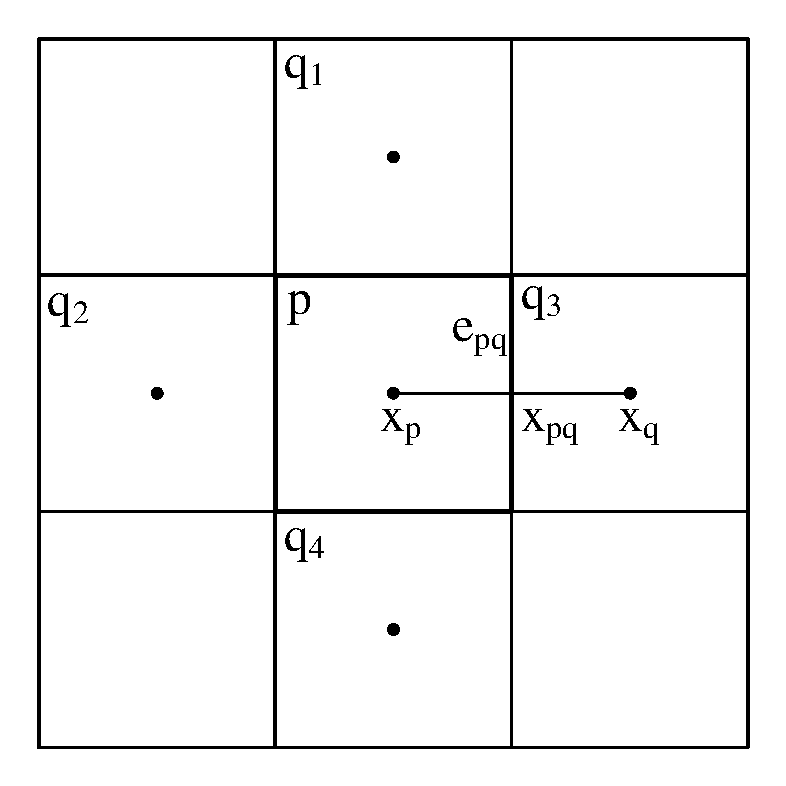
\includegraphics[scale=0.40]{pics/hrany1.pdf}
\caption{Detail siete spolu s označením. V strede sa nachádza pixel $p$, susedné pixle sú označené ako $q_i$, kde $q_i = 1, 2, 3, 4$, hrany medzi pixlami označíme ako $e_{pq}$, $x_p$ a $x_q$ sú body. }
\label{fig:hrany}
\end{center} 
\end{figure}

Pre pixelovú sieť budeme používať označenie uvedené na obr. \ref{fig:hrany}.
Rovnicu (\ref{eq:ihe}) integrujeme cez konečný objem $p$ a dostaneme rovnicu v tvare

\begin{equation} 
\int_p\frac{u^n - u^{n-1}}{\tau} dx = \int_p\nabla . (\nabla u^n)dx.
\end{equation}

Na pravú stranu rovnice aplikujeme Greenovu vetu a dostaneme

\begin{equation} 
\int_p\nabla . (\nabla u^n)dx = \int_{\partial p} \nabla u^n . \vec{n}_pdS,
\end{equation}

kde $\vec{n}_p$ je jednotkovou vonkajšou normálou ku hranici konečného objemu p.
Pretože platí

\begin{equation} 
\int_{\partial p} \nabla u^n \vec{n_p}dS = \sum_{q\in N(p)}\int_{e_{pq}} \nabla u^n . \vec{n}_{pq}dS,
\end{equation}

vieme napísať slabú konečno-objemovú formuláciu úlohy

\begin{equation} 
\int_p\frac{u^n - u^{n-1}}{\tau} dx = \sum_{q\in N(p)}\int_{e_{pq}} \nabla u^n . \vec{n}_{pq}dS = \sum_{q\in N(p)}\int_{e_{pq}} \frac{\partial u^n}{\partial \vec{n}_{pq}} dS,
\end{equation}

Riešenie v MKO chápeme ako po častiach konštantnú funkciu na konečných objemoch $p$, označíme $u_p^n$. Preto vieme ľavú stranu rovnice napísať ako 

\begin{equation} 
\int_p\frac{u^n - u^{n-1}}{\tau} dx = \frac{u^n_q - u^n_p}{\tau} m(p).
\end{equation}

Pravá strana reprezentuje tok (flux) cez hranicu $e_{pq}$ v smere normály $\vec{n}_{pq}$. Člen ľavej strany $\nabla u^n . \vec{n}_{pq}$ aproximujeme na hrane $e_{pq}$ konečnou diferenciou v bode $x_{pq}$ nasledovne

\begin{equation}
\nabla u^n . \vec{n}_{pq} \approx \frac{u^n_q - u^n_p}{d_{pq}}.
\end{equation}

V časovom kroku $n$ aproximáciu $x_{pq}$ použijeme na celej hrane $e_{qp}$ a dostaneme

\begin{equation}
\sum_{q\in N(p)} \int_{e_{pq}} \nabla u^n \vec{n}_{pq} dS \approx \sum_{q\in N(p)} m(e_{pq})\frac{u^n_q - u^n_p}{d_{pq}}.
\end{equation}

Po dosadení dostávame implicitnú schému  

\begin{equation}
\frac{m(p)(u_p^n -u_p^{n - 1})}{\tau} = \sum_{q \in N(p)} m(e_{pq})\frac{(u_q^n - u_p^n)}{d_{pq}}
\end{equation}

kde platia vzťahy $m(p) = h^2, m(e_{pq}) = h, d_{pq} = h$. Po dosadení dostaneme lineárny rovnicový systém

\begin{equation}
u_p^n + \frac{\tau}{h^2}\sum_{q \in N(p)} (u_q^n - u_p^n) = u_p^{n - 1}.
\end{equation}

Pri implicitnej schéme platí bezpodmienečná stabilita (diskrétny princíp minima a maxima), čo znamená, že ak pre ľubovoľnú voľbu priestorového kroku $h$ a časového kroku $\tau$, platí $u_{min} \leq u_p^{n - 1} \leq u_{max}$ potom platí aj pre $u_{min} \leq u_p^{n} \leq u_{max}$. Riešenie lineárneho systému upravíme do nasledovného tvaru

\begin{equation} \label{eq:eihe}
(1 + \frac{\tau}{h^2} \sum_{q \in N(p)}1)u_p^n - \frac{\tau}{h^2} \sum_{q \in N(p)}u_q^n = u_p^{n - 1}.
\end{equation}

Rovnicu (\ref{eq:eihe}) dostaneme na každom konečnom objeme $p$. Následne schému riešime pomocou super-relaxačnej metódy (eng. Successive Over-Relaxation method - SOR). 

\subsection{Numerická schéma pre SUBSURF}

V prvom rade urobíme úpravu do divergentného tvaru, tak že rovnicu (\ref{eq:subsurf}) vydelíme členom $\sqrt{\epsilon^2 + |\nabla u|^2}$ a dostaneme

\begin{equation} \label{eq:cdsubsurf}
\frac{1}{|\nabla u^{n-1}|_{\epsilon}}.\frac{u^n-u^{n-1}}{\tau} = \nabla.(g^0\frac{\nabla u^n}{|\nabla u^{n-1}|_{\epsilon}}),
\end{equation}

kde $g^0 = g(|\nabla G_{\sigma}*I^0|)$ a $|\nabla G_{\sigma}*I^0|$ predstavuje zhľadený gradient. Teraz spravíme priestorovú diskretizáciu pomocou metód konečných objemov, čo znamená, že zintegrujeme rovnicu (\ref{eq:cdsubsurf}) cez konečný objem $p$ a dostaneme

\begin{equation}
\int_{p}\frac{1}{|\nabla u^{n-1}|_{\epsilon}}.\frac{u^n-u^{n-1}}{\tau}dx = \int_{p}\nabla.(g^0\frac{\nabla u^n}{|\nabla u_p^{n-1}|_{\epsilon}})dx,
\end{equation}

Následne na pravú stranu rovnice aplikujeme Greenovu vetu

\begin{equation} \label{greensubsurf}
\int_{p}\frac{1}{|\nabla u^{n-1}|_{\epsilon}}.\frac{u_p^n-u_p^{n-1}}{\tau}dx = \int_{\partial p} g^0\frac{\nabla u^n}{|\nabla u_p^{n-1}|_{\epsilon}}\vec{n_{pq}}_pdS,
\end{equation}

Derivácia v smere vonkajšej normály ku konečnému objemu $p$ je v rovnici (\ref{greensubsurf}) reprezentovaná ako $\nabla u^n.\vec{n_{pq}}$. Na ľavej strane rovnice (\ref{greensubsurf}) budeme uvažovať konštantnú reprezentáciu riešenia a jeho gradientu. Normálovú deriváciu z pravej strany rovnice nahradíme konečnou diferenciou hodnotami, ktoré reprezentujú hodnoty na hranách konečného objemu $p$. Nasledovne

\begin{equation}
\frac{m(p)}{|\nabla u_p^{n-1}|_{\epsilon}}\frac{u_p^n-u_p^{n-1}}{\tau} = \sum_{q \in N(p)}\int_{e_{pq}}g_{pq}^0\frac{u_q^n - u_p^n}{d_{pq}}.\frac{1}{|\nabla u_{pq}^{n-1}|_{\epsilon}}ds.
\end{equation}

Vyčíslením integrálu v časovom kroku $n$ aproximáciu $x_{pq}$ použijeme na celej hrane $e_{qp}$ a dostaneme

\begin{equation} \
\frac{m(p)}{|\nabla u_p^{n-1}|_{\epsilon}}\frac{u_p^n-u_p^{n-1}}{\tau} = \sum_{q \in N(p)}g_{pq}^0\frac{u_q^n - u_p^n}{d_{pq}}.\frac{m(e_{pq})}{|\nabla u_{pq}^{n-1}|_{\epsilon}}.
\end{equation}

Keďže ide o pixelovú sieť s hranu $h$, dostaneme tvar

\begin{equation} \label{sub}
\frac{h^2}{\tau|\nabla u_p^{n-1}|_{\epsilon}}u_p^n + \sum_{q \in N(p)}\frac{g_{pq}^0}{|\nabla u_{pq}^{n-1}|_{\epsilon}}(u_q^n - u_p^n) = \frac{h^2}{\tau|\nabla u_p^{n-1}|_{\epsilon}}u_p^{n - 1}.
\end{equation}

Z tvaru (\ref{sub}), dostaneme rovnicu pre každý pixel

\begin{equation}
a_p^{n - 1}u_p^n - \sum_{q \in N(p)} a_{pq}^{n - 1}u_q^n =b_p^{n-1}u_p^{n-1},
\end{equation}

kde $a_{pq}^{n - 1}, a_p^{n - 1}, b_p^{n - 1}$ označujú

\begin{equation}
\begin{array}{l}
a_{pq}^{n - 1}  = \frac{g_{pq}^{0}}{|\nabla u_{pq}^{n-1}|_{\epsilon}}, \\
a_p^{n - 1} = \frac{h^2}{\tau|\nabla u_p^{n-1}|_{\epsilon}} + \sum_{q \in N(p)} a_{pq}^{n - 1}, \\
b_p^{n - 1} = \frac{h^2}{\tau|\nabla u_p^{n-1}|_{\epsilon}}, \\
\end{array}
\end{equation}

a po dosadení okrajových podmienok dostávame sústavu lineárnych rovníc riešenú v novom časovom kroku $u^n$.

V našom prípade na získanie hranového detektora $g_{pq}^{0}$ použijeme priemer z originálnych dát a dát, na ktoré sme použili niektorú z globálnych alebo lokálnych adaptívnych prahovacích metód nasledovne

\begin{equation}
g_{pq}^{0} = \frac{1}{1 + k|\nabla \frac{u_o + u_t}{2}|^2},
\end{equation}

kde $u_o$ označujú pôvodné dáta a $u_t$ sú vyprahované dáta. 

\newpage
\section{Softvér}

Na implementáciu a vytvorenie prostredia, bol zvolený objektovo orientovaný prístup jazyka C++, spolu s knižnicami Qt \cite{qt}, ktoré obsahujú veľa na implementovaných tried a boli užitočným nástrojom pri vytváraní užívateľského prostredia a VTK \cite{vtk} knižnicami, ktoré slúžia na zobrazovanie a manipuláciu s dátami. 

\subsection{Qt}
Užívateľské rozhranie je vytvorené pomocou Qt knižníc, ktoré sú jedným z najpoužívanejších cross-platformových frameworkov na vytváranie užívateľského prostredia (GUI). Majú aj veľa predprogramovaných knižníc ktoré programátorovi uľahčia prácu. Sú naimplementované v jazyku C++. 

Najčastejšie využívané Qt triedy v projekte:
\begin{itemize}
\item \textbf{QMdiArea}\\ 
Táto trieda zohráva jednu z najdôležitejších funkcií v programe. Funkcie tejto triedy fungujú v podstate ako správca okien pre MDI okná, čo v našom prípade znamená, že umožňuje vytvárať podokná pomocou triedy, v ktorých sa v programe nachádzajú ďalšie Qt triedy slúžiace na vykresľovanie 2D a 3D dát, s ktorými program pracuje. V programe je použité kaskádové usporiadanie takýchto podokien, čo znamená že vykresľovacie okná sa môžu navzájom prekrývať, dajú sa minimalizovať/maximalizovať vrámci hlavného okna a zavrieť.

\item \textbf{QScrollArea} \\
QScrollArea sa nachádza v každom podokne widgetu QMidiArea. Zabezpečuje možnosť priblížiť/oddialiť a posúvať vizualizované dáta. Tiež sa nachádza aj v častiach programu, kde bolo potrebné aplikovať ScrollBar.

\item \textbf{QVTKOpenGLNativeWidget} \\
Widget tejto triedy sa nachádza v každej QScrollAree a umožňuje samotné vykreslenie 2D/3D modelov za pomoci VTK knižníc. 

\item \textbf{QDockWidget} \\
Tento widget obsahuje všetky informácie a nastavenia súvisiace s dátami. Každý logický celok má vlastný panel (\textit{eng.} dock), ktorý sa dá vrámci okna premiestňovať, ukotvovať buď na ľavej alebo na pravej strane okna a v prípade, že sa prekrývajú vytvorí sa z nich viacero záložiek. Taktiež sa dajú v prípade potreby minimalizovať.

\item \textbf{QTreeWidget} \\ 
Všetky dáta, či už pôvodné, vyprahované alebo vysegmentované pomocou programu, sa nachádzajú v zozname, z ktorého sa dá vybrať ktoré dáta budú vykreslené. QTreeWidget bol použitý aby sme vykresľované dáta vedeli zadeliť do medzi  2D alebo 3D dáta.

\item \textbf{QVector} \\
Trieda QVector definuje dynamické polia, je šablónovou triedou.
%, čo znamená že
Ukladá premenné do susedných miesta v pamäti a poskytuje rýchly indexový prístup. Je použitá v prípadoch keď nie je potrebné odstraňovať prvky zvnútra QVectora.

\item \textbf{QFile, QFileDialog} \\
Tieto triedy slúžia v programe na otváranie, načítavanie, ukladanie a manipuláciu s dátami.

\end{itemize}

\subsection{VTK}

Visualization Toolkit (VTK) sú voľne dostupnými knižnicami, ktoré v programe slúžia na zobrazovanie a interakciu s 2D aj 3D dátami. Spomenieme niektoré knižnice, ktoré hrajú dôležitú úlohu pri našej implementácii.

\begin{itemize}
\item \textbf{vtkSmartPointer} \\
Táto šablónová trieda, slúži ako pointer pre VTK triedy. Jeho úlohou je zlepšiť manažment s pamäťou, čo znamená, že v prípade ak sú dáta mimo rozsahu alebo sa nikde nepoužívajú tak budú automaticky odstránené. Teda uľahčuje pracovať s dátami bez varovných hlášok.

\item \textbf{vtkPoints} \\
Je triedou reprezentujúcou zoskupenie trojíc $(x, y, z)$ 3D bodov a manipuláciou s uloženými bodmi.
 
\item \textbf{vtkPolygon} \\
Uľahčuje vytváranie buniek $n$-stranného mnohouholníka v rovine. V našom prípade ide o štvoruholníky, znázorňujúce diskrétnu sieť. Každý štvoruholník reprezentuje jeden pixel načítaných obrazových dát.     
 
\item \textbf{vtkTriangles} \\
Umožňuje vytvorenie trojuholníkových buniek v priestore.

\item \textbf{vtkCellArray} \\
Objekty triedy vtkCellArray zabezpečujú prepojenie samostatných buniek rôznych typov, v našej implementácii sa jedná o bunky trojuholníkové (vtkTriangles) a štvorcové (vtkPolygon). Štruktúra tejto triedy je reprezentovaná celočíselným poľom so štruktúrou v tvare: $(n,id_1,id_2, \dots,id_n, n,id_1,id_2, \dots,id_n, \dots)$, kde $n$ je počet bodov, nachádzajúcich sa v bunke a $id$ je index z pridruženého zoznamu bodov.

\item \textbf{vtkPolyData} \\
V objektoch tejto triedy sú zadefinované vykresľované dáta, či už sa jedná o 2D alebo 3D dáta. V tejto triede môžu byť uložené informácie o tom akým spôsobom budú dáta reprezentované - geometrické informácie o štruktúre vykresľovaných dát. Takýmito informáciami môžu byť napríklad body, bunky, vektory, čiary, polygonálne alebo trojuholníkové pásy.

\item \textbf{vtkColorTransferFunction} \\
Je to trieda, ktorá nám slúži na definíciu farebných prechodov cez farebné modely RGB alebo HSV v počastiach spojitom priestore. 

\item \textbf{vtkPolyDataMapper} \\
Je triedou, zabezpečujúcou tzv. 'namapovanie' čo znamená, že zadefinuje, vlastnosti polydát definovaných ako objekt triedy vtkPolyData, ktoré sú potrebné pri následnom vykreslení.

\item \textbf{vtkActor} \\
Táto trieda reprezentuje, geometriu a vlastnosti vykresľovaných dát na zobrazovanej scéne. Odkazuje na geometriu uloženú ako objekt triedy na vtkPolyDataMapper a dedí funkcie súvisiace s pozíciou a orientáciou vykresľovaných dát. Tieto informácie sú uložené v transformačnej matici o veľkosti $4x4$, ktorá zabezpečuje rotácie vo všetkých smeroch $(x, y, z)$, škálovanie objektov atď..

\item \textbf{vtkRenderer} \\
Trieda zabezpečujúca samotné vykresľovanie dát. Stará sa o prevod geometrie, špecifikuje svetelné podmienky a orientáciu kamery. Tiež vykonáva transformáciu súradníc medzi svetovými súradnicami, súradnicami zobrazenia (t.j. súradnicový systém počítačovej grafiky) a súradnicami displeja (t.j.  súradnice obrazovky displeja).

\item \textbf{vtkCutter} \\
Trieda vtkCutter, je filtrovacou triedou, ktorá pomocou implicitnej funkcie zabezpečuje vykresľovanie, viacerých alebo jedného rezu cez trojdimenzionálne dáta. Vo VTK na rezanie (eng. cutting) znamená zredukovanie dimenzie o jedna. V našom prípade išlo o 3D dáta, ktoré sme rezali pomocou roviny. 

\item \textbf{vtkCubeAxesActor} \\
Pomocou tejto triedy, sú zobrazované hranice vykresľovaných dát spolu s označeniami osí a  hodnotami nachádzajúcimi sa v smeroch $x, y, z$ - výška, šírka a hĺbka.

\item \textbf{vtkInteractorStyleJoystickCamera}, \textbf{vtkInteractorStyleImage}  \\
Tieto dve triedy umožňujú prepínanie interakcie objektu s prostredím, v našom prípade išlo o odobranie možnosti rotácie pri 2D obrazových dátach.

\item \textbf{vtkXMLPolyDataWriter} \\
Extrahuje dáta typu vtkPolydata do súboru. Štandardný formát vytvoreného súboru je \textit{.vtp}. 
\end{itemize}

\subsection{Rozdelenie projektu do tried}

Projekt je rozdelený do viacerých súborov(tried) dodržiavajúcej zásady objektovo-orientovaného programovania, z ktorých každá zabezpečuje funkcionalitu inej časti programu. Nasledovne:

\begin{itemize}
\item Trieda \textbf{bioData}, spája všetky triedy a definuje užívateľské rozhranie pomocou Qt knižníc.
\item V \textbf{source} sa načítavajú dáta zo súborov, vytvárajú sa dáta na následné zobrazenie spolu so zafarbením. Taktiež obsahuje funkcie na uloženie dát v rôznych formátoch.    
\item V triede \textbf{filters}, sú definované všetky prahovacie a segmentačné metódy.
\item \textbf{ViewerWidget} zabezpečuje vykresľovanie samotných 2D aj 3D dát, spolu s osami a izočiarami. 
\item Trieda \textbf{subWin} uchováva, hodnoty nastavené v užívateľskom rozhraní pre každé otvorený súbor osobitne.

\end{itemize}


\subsection{Grafické užívateľské rozhranie}

V tejto sekcii sa oboznámime s vizuálnou stránkou vytvoreného softvéru a popíšeme funkcionalitu. Pri tvorbe programu sme sa zamerali na to aby bol čo najjednoduchší a vedel ho ovládať aj niekto, kto sa do danej problematiky až tak do hĺbky nevyzná. Grafické rozhranie(GUI) je vytvorené pomocou Qt knižníc.

Pri otvorení programu sa zobrazí okno, v ktorom sa nachádza horná lišta s položkami File, Settings a Help zvyšok bude načítaný až po otvorení. V každej z týchto položiek sa nachádzajú ďalšie možnosti. Položka File obsahuje možnosti: Open, Save, Close Files a Close.

\begin{figure}[h!]
 \begin{center} 
 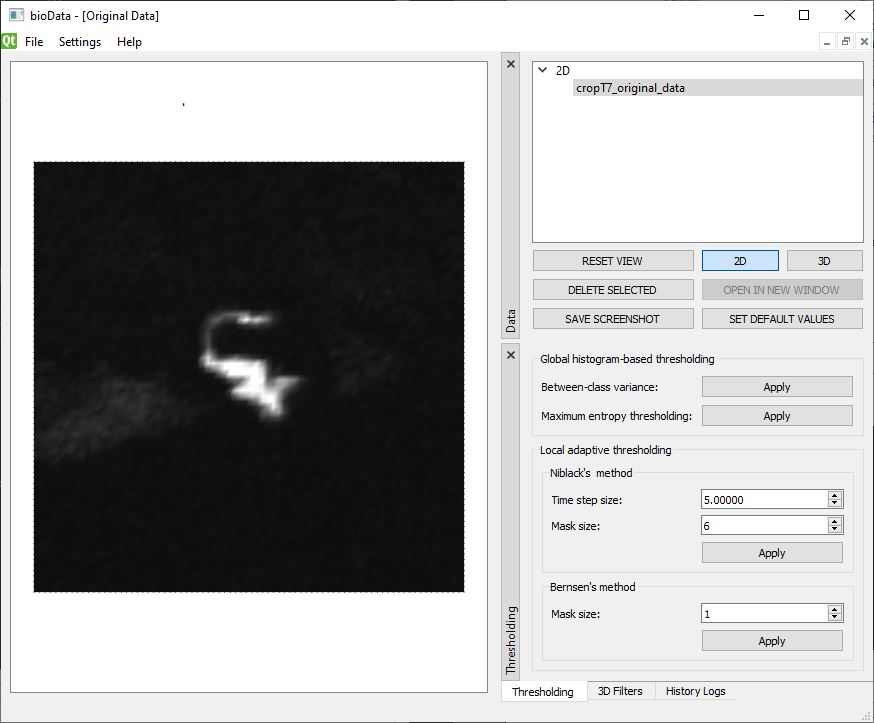
\includegraphics[scale=0.50]{pics/ui1.jpg}
\caption{Grafické rozhranie programu po načítaní vybraných dát.}
\label{fig:ui1}
\end{center} 
\end{figure}

Po zvolení možnosti Open, sa otvorí dialógové okno, z ktorého sa dajú vybrať obrazové súbory typu .pgm (portable gray map). Po zvolení súboru sa zobrazí celé užívateľské prostredie aj so zvolenými dátami obr. \ref{fig:ui1}. Na ľavej strane sú zobrazené načítané dáta. Na pravej strane, môžeme vidieť bočný panel rozdelený na dve časti, v ktorých sa nachádza zoznam spracovávaných dát v programe pre 2D aj 3D dáta, možnosti pre 2D a 3D dáta spolu so všetkými implementovanými filtrami, prahovacími metódami a možnosťami pre zobrazenie uložených vo viacerých záložkách. 

Prvá časť panelu má názov \textit{Data} obr. \ref{fig:uidata}a obsahuje zoznam 2D a 3D dát, s ktorými sa doteraz pracovalo. Umožňuje spätné načítanie dát nachádzajúcich sa v zozname. Tiež obsahuje tlačidlá: 
\begin{itemize}
\item \texttt{RESET VIEW} - vykresľovaný objekt, prekreslí na stred vykresľovacej plochy.  
\item \texttt{2D} - v prípade, že v zozname sú zvolené 2D dáta, odoberie možnosť rotácie a je vysvietené.
\item \texttt{3D} - v prípade, že v zozname sú zvolené 3D dáta, tak sa s nimi dá adekvátne manipulovať a tlačidlo je vysvietené.
\item \texttt{DELETE SELECTED} - vymaže zvolené dáta zo zoznamu.
\item \texttt{OPEN IN NEW WINDOW} - zatiaľ neaktívne.
\item \texttt{SAVE SCREENSHOT} - uloží práve zobrazené dáta z vykresľovacej plochy ako obrazové dáta vo formáte \textit{.png}
\item \texttt{SET DEFAULT VALUES} - prestaví hodnoty všetkých voliteľných hodnôt naspäť na predvolené hodnoty.
\end{itemize}

V záložke \texttt{Thresholding} obr. \ref{fig:uidata}b, sa nachádzajú štyri implementované prahovacie algoritmy, ktoré vstupujú  následne ako okrajová podmienka do segmentačnej metódy. Ide o dva globálne prahovacie algoritmy, ktoré závisia len na histograme a teda neberú na vstup žiadne parametre. A dva lokálne adaptívne prahovacie algoritmy, ktoré berú na vstup veľkosť masky a jeden z nich veľkosť časového kroku.


\begin{figure}[H]%
    \begin{center} 
    \subfloat[Detail docku \texttt{Data}.]{{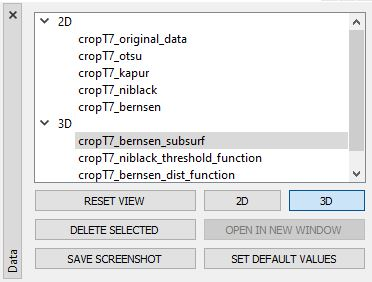
\includegraphics[scale=0.65]{pics/uidata.jpg} }}%
    \qquad
    \subfloat[Detail docku \texttt{Thresholding}.]{{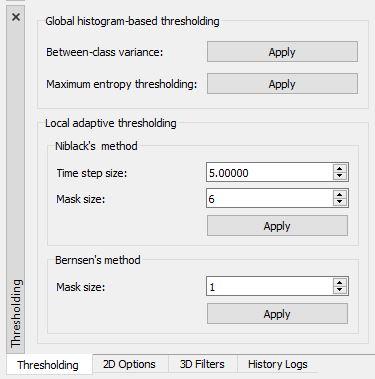
\includegraphics[scale=0.55]{pics/uithr.jpg} }}%
    \caption{}%
    \label{fig:uidata}%
     \end{center} 
\end{figure}

Záložka \texttt{2D Options} obr. \ref{fig:uidata1}a je zobrazená len v prípade, že sú zvolené 2D dáta. V tejto záložke sa nachádzajú možnosti súvisiace len s 2D dátami. Dájú sa tam zobraziť kontúry na dátach,  jeden krok rovnice vedenia tepla a priemer originálnych a vyprahovaných obrazových dát. 

\texttt{3D Filters} obr. \ref{fig:uidata1}b obsahuje možnosti pre samotný SUBSURF spolu s jeho parametrami. Taktiež sa tam nachádzajú počiatočné podmienky znamienkovej dištančnej a prahovacej funkcie, ktoré sa dajú zobraziť ešte pred vstupom do SUBSURFu.


\begin{figure}[H]%
    \centering
    \subfloat[Detail docku \texttt{2D Options}.]{{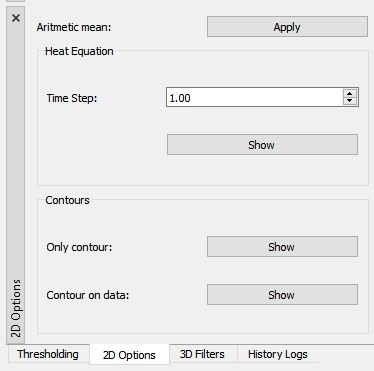
\includegraphics[scale=0.65]{pics/ui2Dopt.jpg} }}%
    \qquad
    \subfloat[Detail docku \texttt{3D Filters}.]{{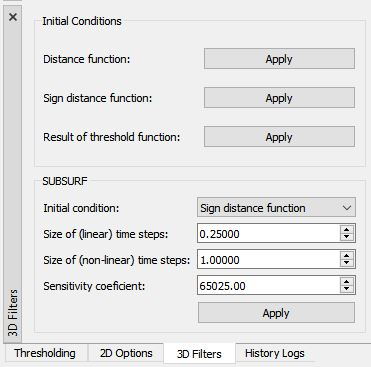
\includegraphics[scale=0.65]{pics/ui3Dfilt.jpg} }}
    \caption{}%
    \label{fig:uidata1}%
\end{figure}

V \texttt{3D Options} obr. \ref{fig:uidata2}a je zobrazený len v prípade, že sú zvolené 3D dáta. V tejto záložke sa nachádzajú možnosti súvisiace len s 3D dátami. V týchto možnostiach sa dajú zapnúť osi, zmeniť farba, vykresliť zvolený počet izočiar buď na dátach alebo bez nich a dá sa zvoliť optimálna izočiara a následne ju je možné vykresliť na pôvodných dátach. 

\begin{figure}[H]%
    \centering
    \subfloat[Detail docku \texttt{3D Options}.]{{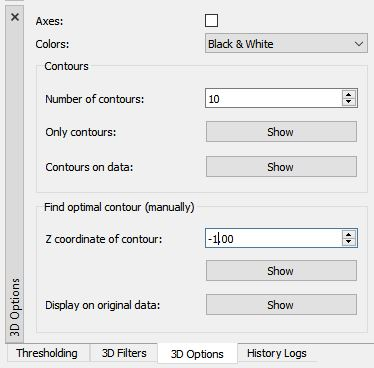
\includegraphics[scale=0.65]{pics/ui3Dopt.jpg} }}%
    \qquad
    \subfloat[Detail docku \texttt{History Logs}.]{{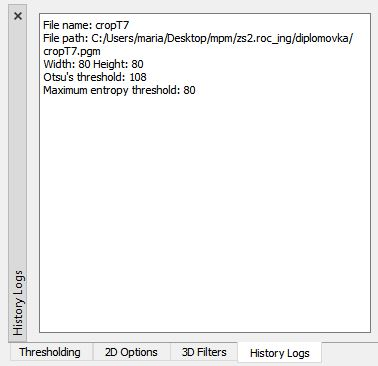
\includegraphics[scale=0.65]{pics/uihist.jpg} }}
    \caption{}%
    \label{fig:uidata2}%
\end{figure}

V záložke \texttt{History Logs} obr. \ref{fig:uidata2}b sa nachádza jednoduché textové pole, ktoré zaznamenáva väčšinu úkonov vykonaných v programe. Taktiež sa tam nachádzajú informácie o načítanom súbore, ako napríklad aj názov súboru, cesta k súboru atď... Tento výstup sa dá uložiť do jednoduchého textového súboru.

Na obr. \ref{fig:uidata3}a sú zobrazené dáta s makrofágom, na ktoré bol aplikovaný SUBSURF, za počiatočnú podmienku bola použitá dištančná funkcia.

\begin{figure}[H]%
    \centering
    \subfloat[Grafické rozhranie programu zobrazujúce 3D dáta spolu s osami x,y,z.]{{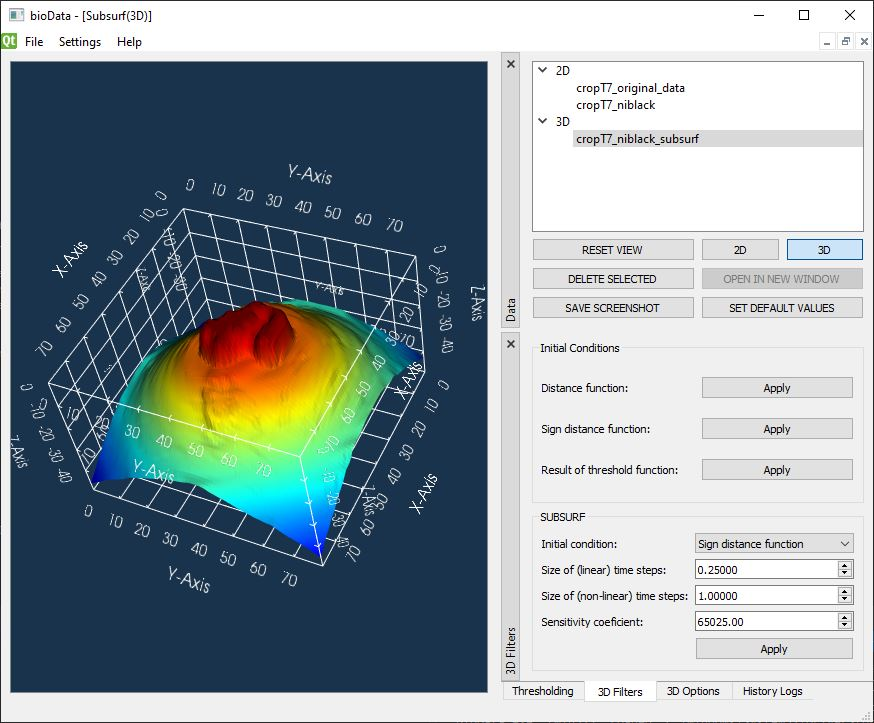
\includegraphics[scale=0.3]{pics/subsurf.jpg} }}%
    \qquad
    \subfloat[Grafické rozhranie programu zobrazujúce výslednú izočiaru na pôvodných dátach]{{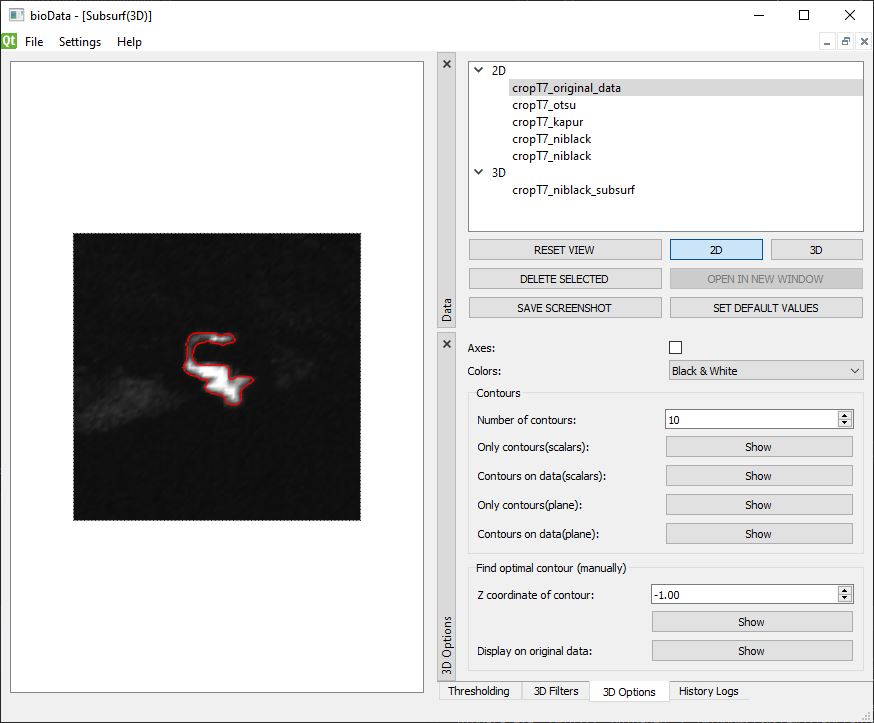
\includegraphics[scale=0.3]{pics/result.jpg} }}%
    \caption{}%
    \label{fig:uidata3}%
\end{figure}


Na obr. \ref{fig:uidata3}b sú vidieť pôvodné dáta, na ktorých je zobrazená výsledná izočiara.

Vykresľovacia plocha má niekoľko, vstavaných funkcií, ktoré sa dajú ovládať cez klávesové skratky. Ide napríklad o klávesy \texttt{W} a \texttt{S} prepínajú zobrazenie dát medzi obrysom dát a zafarbeným modelom, klávesa \texttt{R} reštartuje pohľad na objekt na vykresľovanej ploche.
 
Zvyšné možnosti, v hornej lište v položke \texttt{File} sa ešte nachádza možnosť \texttt{Save}, ktorá ponúka buď exportovanie 2D aj 3D dát vo VTK formáte \textit{.vtp} (typ súboru špecifický pre vtkPolyData) alebo 2D dáta vie uložiť ako ascii portable gray map dáta \textit{.pgm}. Ďalšou možnosťou je \texttt{Close Files}, kedy sa zatvoria všetky otvorené súbory. A možnosti \texttt{Close}, ktorá zatvorí celý program.

V hornej lište sa ešte nachádzajú položky \texttt{Settings} a \texttt{Help}. V \texttt{Settings} vie užívateľ skryť/zobraziť všetky položky nachádzajúce sa vpravo. A \texttt{Help} obsahuje informácie o programe a jednoduchú dokumentáciu.

\subsection{Príklad použitia}

V tejto časti si ukážeme príklad na použitie implementovaného softvéru. Otvoríme súbor typu \textit{.pgm}. Načíta sa uŽívateľské prostredie obr. \ref{fig:ui1}. V záložke \texttt{Thresholding}, zvolíme niektorú z implementovaných prahovacích funkcií, v tomto príklade zvolíme Niblackovu metódu, s časovým krokom $sigma = 50.0$ a veľkosťou masky $m = 3$. Výsledok prahovania v užívateľskom prostredí je zobrazený na obr \ref{fig:nbui}.

 
\begin{figure}[H]
 \begin{center} 
 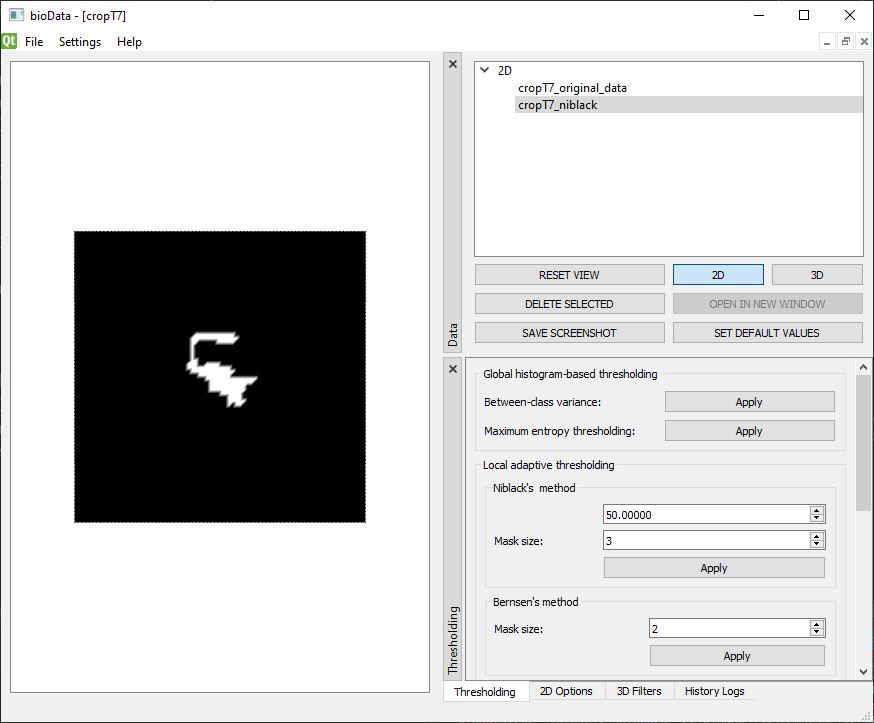
\includegraphics[scale=0.50]{pics/uinb.jpg}
\caption{Grafické rozhranie, s dátami na ktorých je aplikovaná Niblackova prahovacia metóda.}
\label{fig:nbui}
\end{center} 
\end{figure}

Vyprahované dáta, boli pridané do zoznamu. Tieto dáta použijeme na vstup do segmentačnej metódy SUBSURF. Zvolíme záložku \texttt{3D Filters} detail možností je zobrazený na obr. \ref{fig:uidata1}b, kde sa dajú zobraziť 2 funkcie, ktoré môžeme použiť ako počiatočnú podmienku do segmentačnej metódy. Prvou možnosťou počiatočnej podmienky  je znamienková funkcia vzdialenosti obr. \ref{fig:pp}a. Druhá možnosť je výsledok prahovacej funkcie  obr. \ref{fig:pp}b, čo znamená, že takéto dáta majú nastavené súradnice $z$ na $-1$, ak prahovacia funkcia zaradila pixel do pozadia a $1$, ak sa jedná o pixel makrofágu. Prahovacia funkcia idúca na vstup, musí byť v oboch prípadoch vyznačená v paneli \texttt{Data}.


\begin{figure}[H]%
    \centering
    \subfloat[Grafické rozhranie programu zobrazujúce znamienkovú funkciu vzdialenosti spolu s osami x,y,z.]{{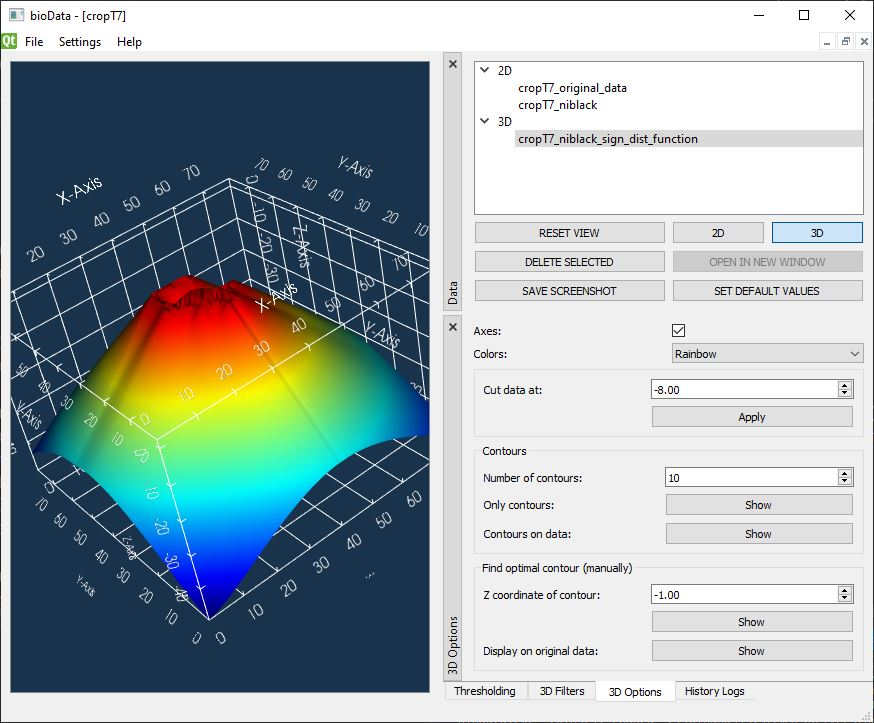
\includegraphics[scale=0.3]{pics/sdf.jpg} }}%
    \qquad
    \subfloat[Grafické rozhranie programu zobrazujúce prahovaciu funkciu.]{{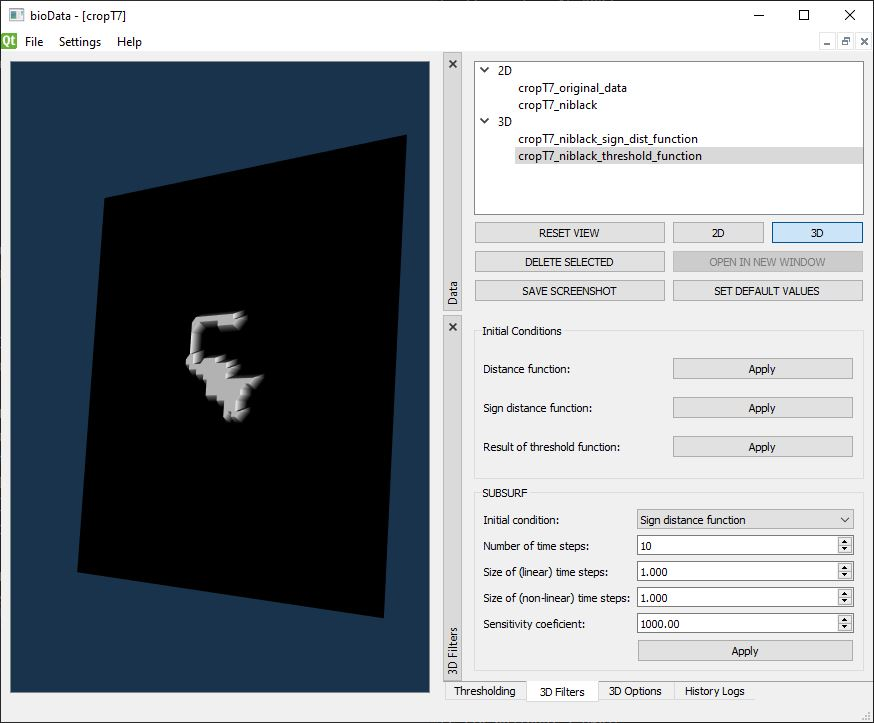
\includegraphics[scale=0.3]{pics/tf.jpg} }}%
    \caption{}%
    \label{fig:pp}%
\end{figure}

Typ počiatočnej podmienky, vstupujúcej do segmentačnej metódy SUBSURF zvolíme zo zoznamu. Nálsledne nastavíme požadované parametre metódy: počet časových krokov $t$, veľkosť lineárneho časového kroku $\sigma$, veľkosť nelineárneho časového kroku $\tau$, koeficient sensitivity $k$. V ukážkovom príklade obr. \ref{fig:res_subsurf} sú použité hodnoty: $t = 10$, $\sigma = 0.25$, $\tau = 1.0$, $k = 200$, pre oba druhy počiatočných podmienok. 


\begin{figure}[H]%
    \centering
    \subfloat[Grafické rozhranie a výsledok segmentačnej funkcie pri použití znamienkovej funkcie vzdialenosti pre počiatočnú podmienku.]{{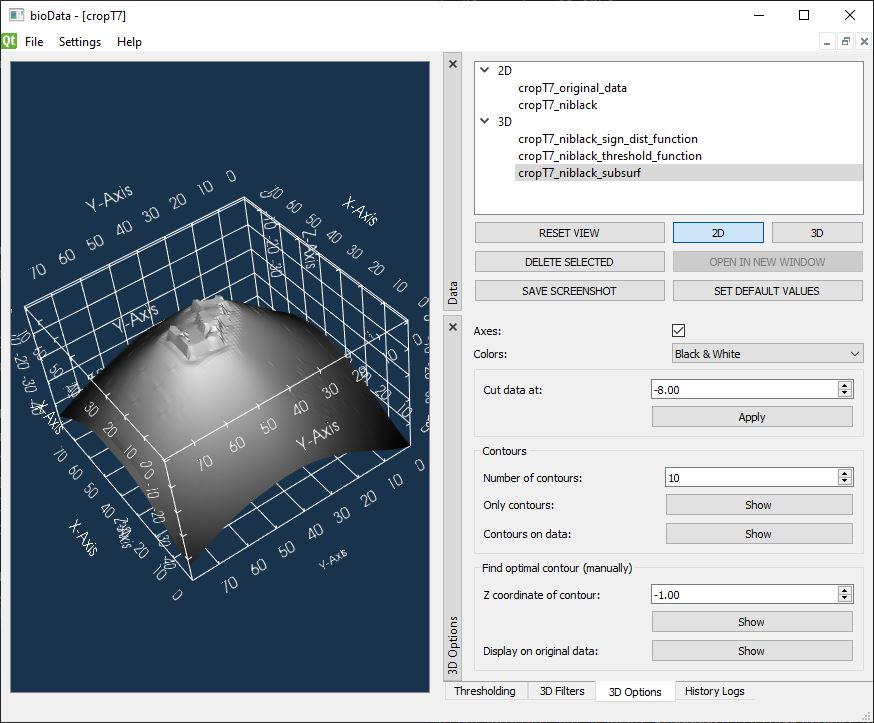
\includegraphics[scale=0.3]{pics/res_sdf.jpg} }}%
    \qquad
    \subfloat[Grafické rozhranie a výsledok segmentačnej funkcie pri použití prahovacej funkcie pre počiatočnú podmienku.]{{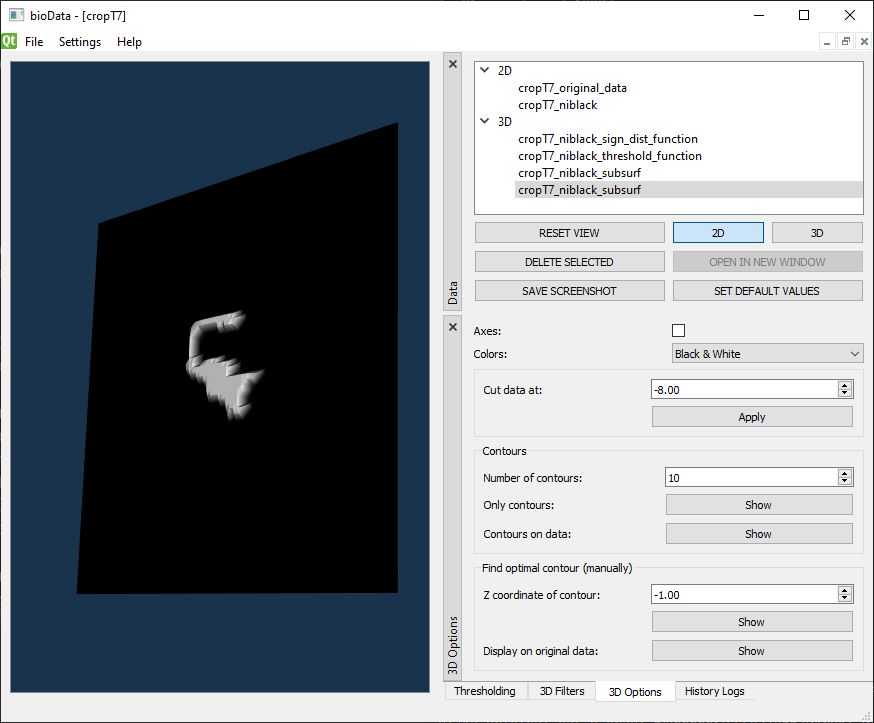
\includegraphics[scale=0.3]{pics/res_tf.jpg} }}%
    \caption{}%
    \label{fig:res_subsurf}%
\end{figure}

Na obr. \ref{fig:res_subsurf}a je zobrazený výsledok s počiatočnou podmienkou znamienkovej funkcie vzdialenosti, kde si môžeme všimnúť, že približne od hodnoty $-10$ neovplyvní výsledok segmentácie, preto ju orežeme na zvolenej hodnote a všetky hodnoty sa nachádzajúce sa pod ňou budú mať hodnotu $-10$.  Možnosť na orezanie dát sa nachádza v záložke \texttt{3D Options} obr. \ref{fig:uidata2} a výsledok je zobrazený na obr. \ref{fig:res_cut}. 

 
\begin{figure}[H]
 \begin{center} 
 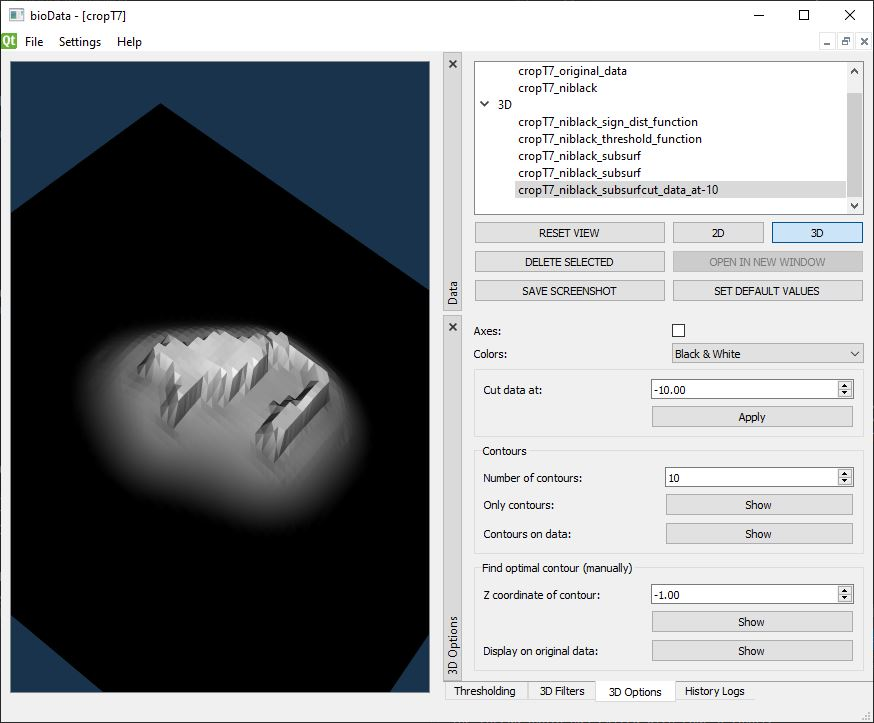
\includegraphics[scale=0.50]{pics/res_cut_sdf.jpg}
\caption{Grafické rozhranie, s orezanými dátami.}
\label{fig:res_cut}
\end{center} 
\end{figure}

Teraz zvolíme optimálnu izočiaru, v prípade počiatočnej podmienky znamienkovej funkcie vzdialenosti zvolíme izočiaru s hodnotou $z = -1.5$ obr. \ref{fig:res_iso}a. V prípade počiatočnej podmienky prahovacej funkcie bude mať izočiara hodnotu $z = 0$ obr. \ref{fig:res_iso}b. 

\begin{figure}[H]%
    \centering
    \subfloat[Grafické rozhranie, výsledok segmentačnej funkcie pri použití znamienkovej funkcie vzdialenosti pre počiatočnú podmienku a izočiara na hodnote $z = -1.5$ .]{{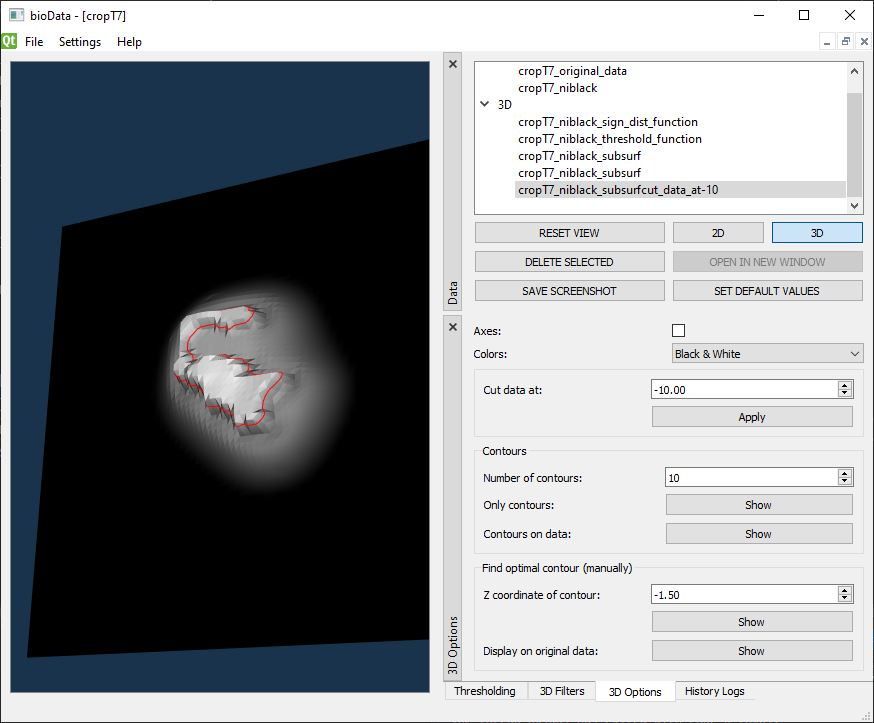
\includegraphics[scale=0.3]{pics/res_iso_3sdf.jpg} }}%
    \qquad
    \subfloat[Grafické rozhranie, výsledok segmentačnej funkcie pri použití prahovacej funkcie pre počiatočnú podmienku a izočiara na hodnote $z = -1.5$.]{{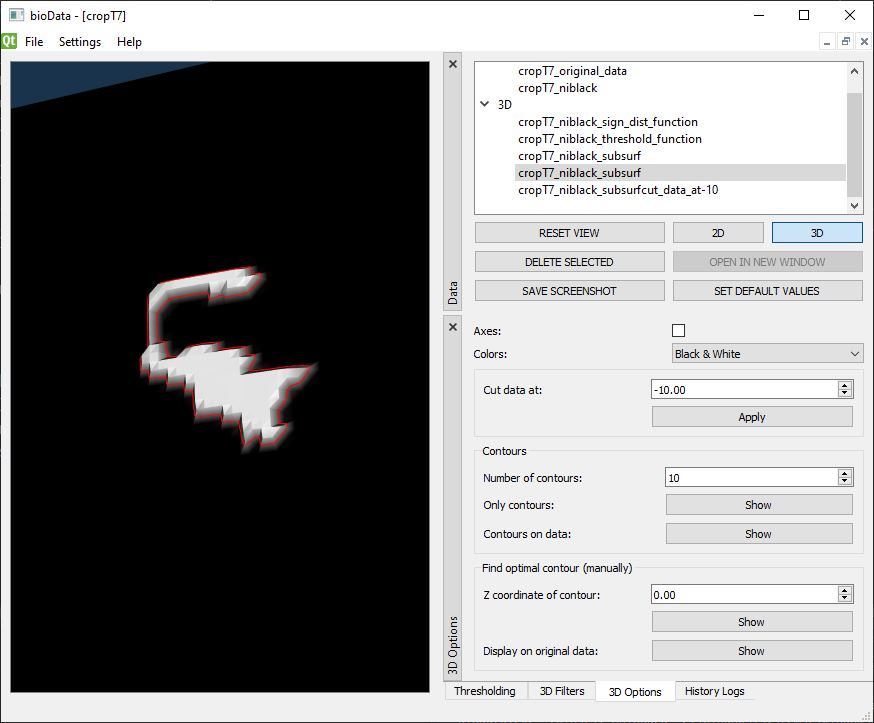
\includegraphics[scale=0.3]{pics/res_iso_3tf.jpg} }}%
    \caption{}%
    \label{fig:res_iso}%
\end{figure}

Nakoniec optimálne zvolenú izočiaru vykreslíme  obr. \ref{fig:res_iso_final} spolu s pôvodnými dátami. Výsledné dáta vieme uložť pomocou \texttt{SAVE SCREENSHOT} tlačidla vo formáte \textit{.png}. 

\begin{figure}[H]%
    \centering
    \subfloat[Grafické rozhranie, výsledná izočiara na pôvodných.]{{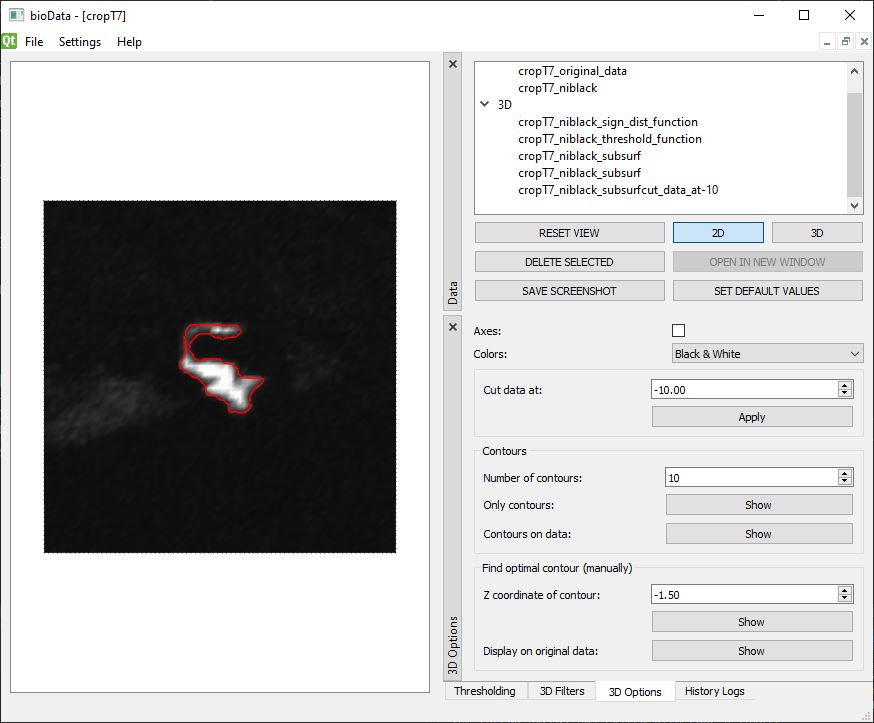
\includegraphics[scale=0.3]{pics/res_iso_sdf.jpg} }}%
    \qquad
    \subfloat[Grafické rozhranie a výsledok segmentačnej funkcie pri použití prahovacej funkcie pre počiatočnú podmienku.]{{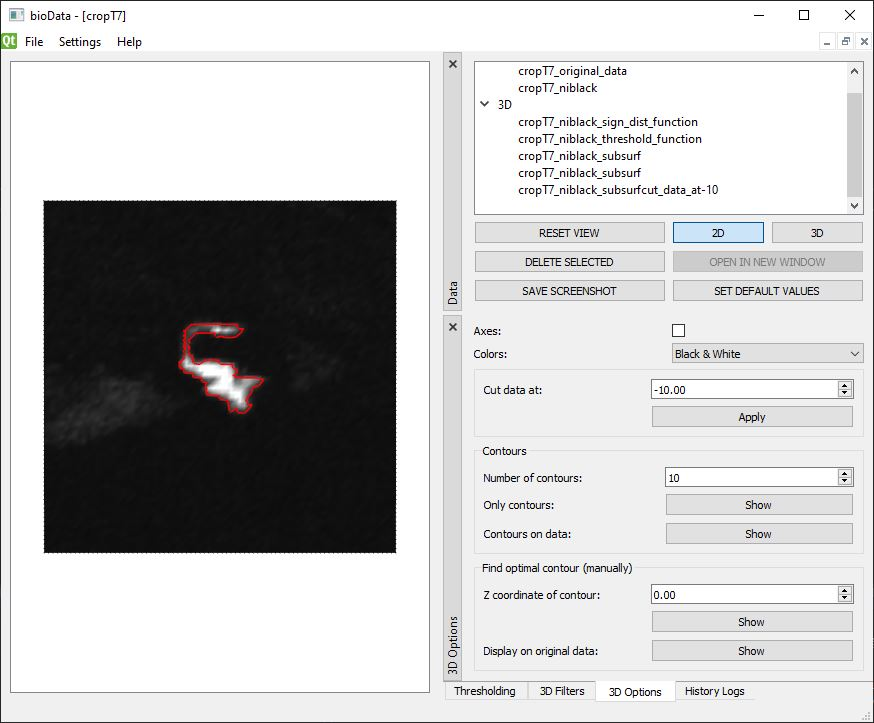
\includegraphics[scale=0.3]{pics/res_iso_tf.jpg} }}%
    \caption{}%
    \label{fig:res_iso_final}%
\end{figure}


\newpage
\section{Výsledky}

Na ukážku výsledkov sme vybrali niekoľko dát s makrofágmi so zložitými tvarmi a šumom v pozadí. Vybrali sme nasledujúce dáta. Obr. \ref{fig:ogData}a bol vybraný z dôvodu, že niektoré časti sú 'odtrhnuté' od zvyšku maktofágu  a dáta obsahujú výrazný šum, viditeľný priamo za makrofágom. Dáta na Obr. \ref{fig:ogData}b a Obr. \ref{fig:ogData}c majú užšie časti, so slabšími intenzitami, ktoré je tiež potrebné zahrnúť ako časť makrofágu. Dáta \ref{fig:ogData}d majú na ľavej časti výrazne slabšiu intenzitu.

\begin{figure}[h!]  
 \subfloat[cropT2]   
   {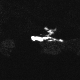
\includegraphics[scale=1.71]{pics/cropT2.png}}
    \hspace{5px}
     \subfloat[cropT7] 
    {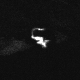
\includegraphics[scale=1.71]{pics/cropT7.png}}
    \hspace{5px}
     \subfloat[cropT27] 
    {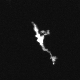
\includegraphics[scale=1.71]{pics/cropT27.png}}
    \hspace{5px}
     \subfloat[cropT45] 
    {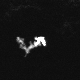
\includegraphics[scale=1.71]{pics/cropT45.png}}
    \caption{Zvolené originálne dáta.}
    \label{fig:ogData}
\end{figure}

Na vstup do segmentačnej metódy sme použili dva druhy počiatočných podmienok a niekoľko prahovacích metód popísaných v sekcii \ref{math}. Úlohou bolo, nájsť počiatočnú podmienku spolu s prahovacou metódou, ktoré by čo najpresnejšie popisovali pôvodný tvar makrofágu. Parametre segmentačnej metódy SUBSURF boli zvolené nasledovne:
$t = 15, \sigma = 0.25, \tau = 1.0, k = 200$ a hodnotu výslednej izočiary sme volili podľa toho aký typ počiatočnej podmienky bol zvolený. Pri počiatočnej podmienke danej znamienkovou funkciou vzdialenosti sme izočiaru nastavili na hodnotu $z = -1$ a pri počiatočnej podmienke danej prahovacou funkciou bola izočiara nastavená na $z = 0$, keďže vo väčšine prípadoch boli tieto voľby najvhodnejšími. Výsledky segmentácie sú vyznačené na pôvodných dátach červenou farbou. 

%\subsection{Globálne prahovanie}

Na obr. \ref{fig:otsu} je zobrazená globálna prahovacia funkcia popísaná v sekcii \ref{OtsuM} používajúca Otsuho metódu. Dá sa všimnúť, že táto prahovacia metóda nezachytila celý tvar makrofágu, hlavne ak išlo o úzku časť s menšou intenzitou.

\begin{figure}[H]  
 \subfloat[cropT2: ]   
   {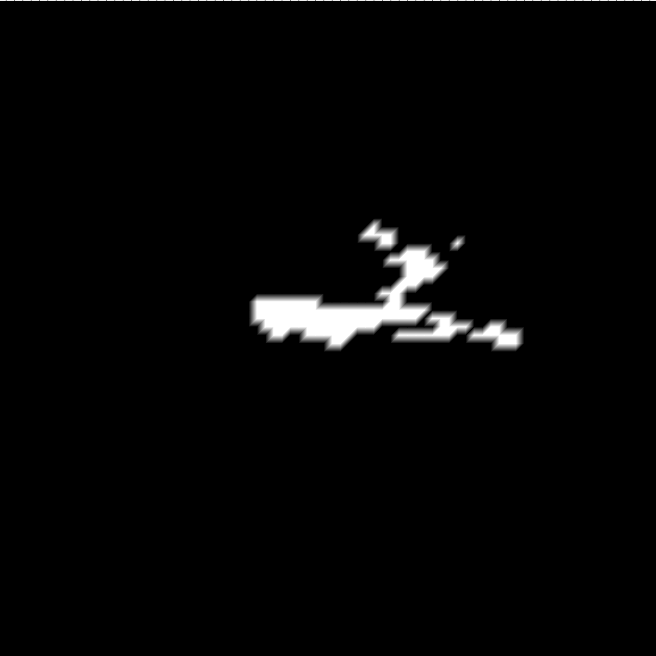
\includegraphics[scale=0.21]{pics/cropT2_otsu.png}}
    \hspace{5px}
     \subfloat[cropT7] 
    {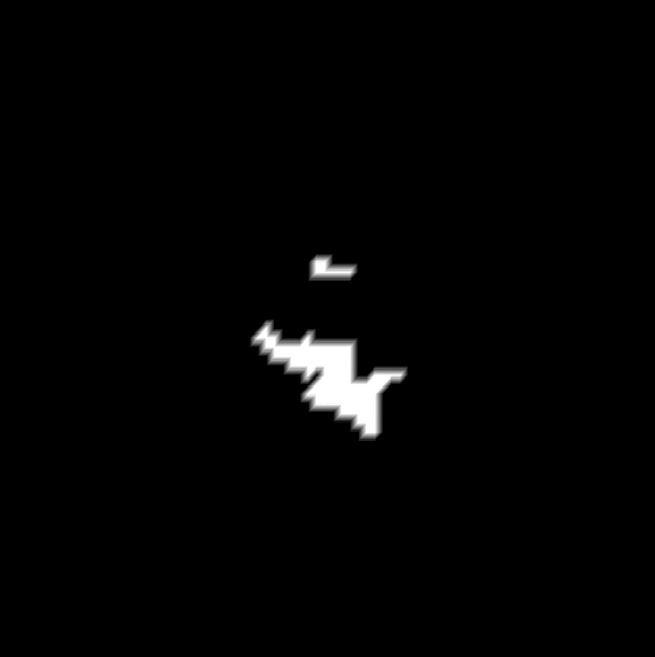
\includegraphics[scale=0.21]{pics/cropT7_otsu.png}}
    \hspace{5px}
     \subfloat[cropT27] 
    {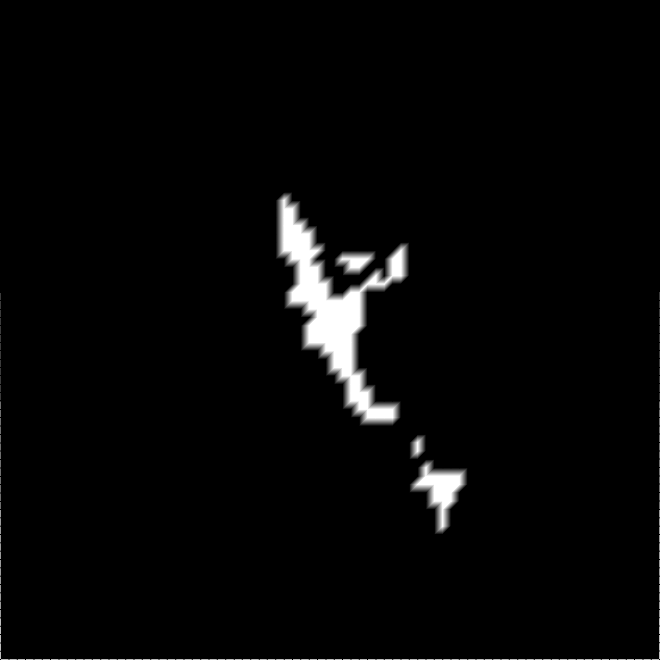
\includegraphics[scale=0.21]{pics/cropT27_otsu.png}}
    \hspace{5px}
     \subfloat[cropT45: prah = 105] 
    {
\includegraphics[scale=0.21]{pics/cropT45_otsu.png}}
    \caption{Otsuho metóda}
    \label{fig:otsu}
\end{figure}

Izočiara na obr. \ref{fig:otsu_sdf} vyznačujúca výsledok segmentácie s počiatočnou podmienkou znamienkovej funkcie vzdialenosti. Môžeme si všimnúť, že niektoré časti makrofágu odtrhnuté aplikáciou prahovacej metódy, sa segmentáciou spätne spojili. 

\begin{figure}[H]  
 \subfloat[cropT2]   
   {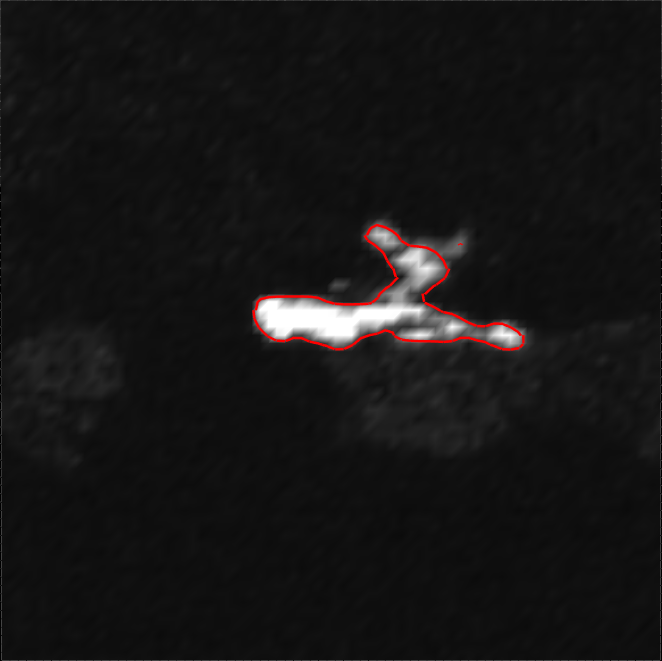
\includegraphics[scale=0.21]{pics/cropT2_otsu_sdf.png}}
    \hspace{5px}
     \subfloat[cropT7] 
    {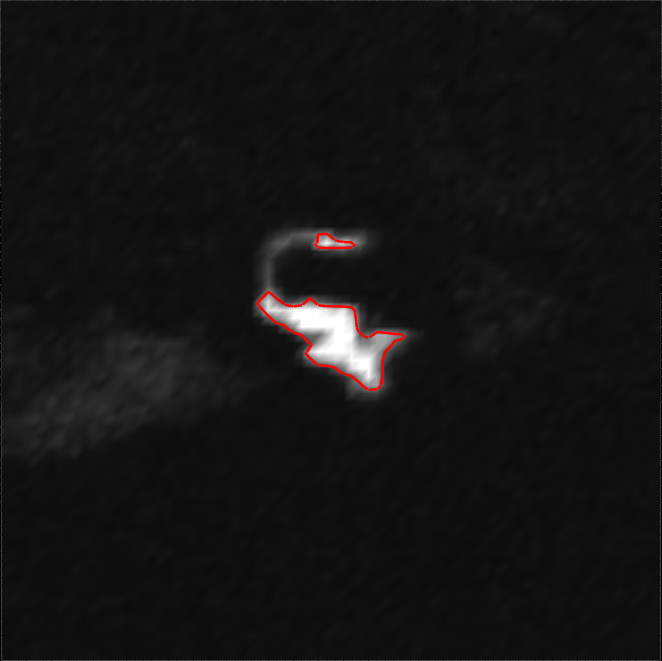
\includegraphics[scale=0.21]{pics/cropT7_otsu_sdf.png}}
    \hspace{5px}
     \subfloat[cropT27] 
    {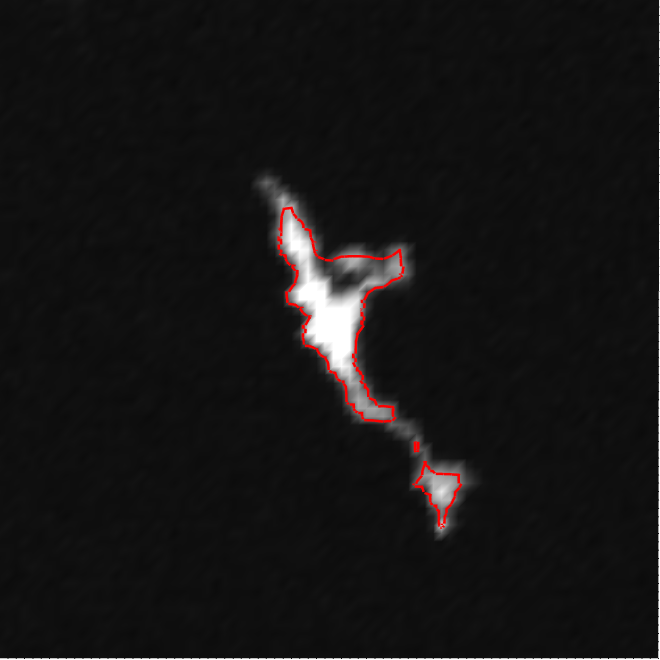
\includegraphics[scale=0.21]{pics/cropT27_otsu_sdf.png}}
    \hspace{5px}
     \subfloat[cropT45] 
    {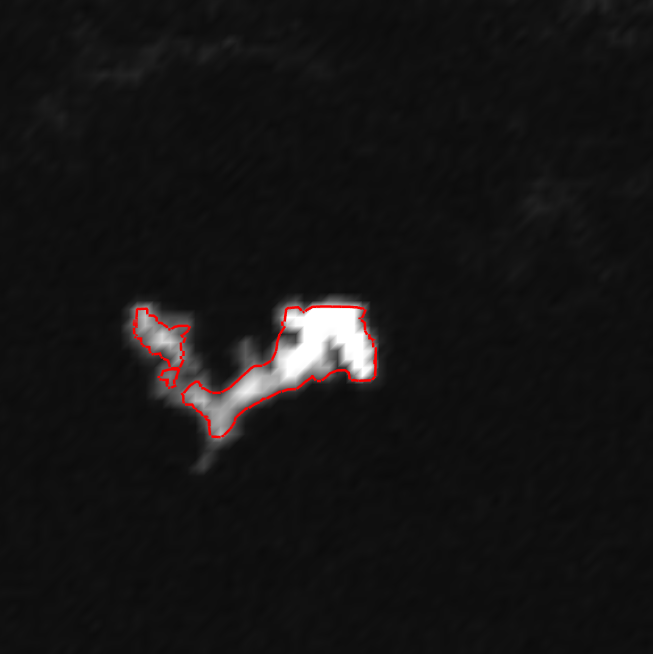
\includegraphics[scale=0.21]{pics/cropT45_otsu_sdf.png}}
    \caption{Výsledok segmentácie. Použitá Otsuho metóda a znamienková funkcia vzdialenosti.}
    \label{fig:otsu_sdf}
\end{figure}

Na obr. \ref{fig:otsu_tf} vidíme výsledok segmentačnej metódy s počiatočnou podmienkou vytvorenej z prahovacej metódy. Tato počiatočná podmienka nevylepšila výsledok, výsledky sú takmer totožné s s výsledkom prahovacej metódy. 

\begin{figure}[H]  
 \subfloat[cropT2]   
   {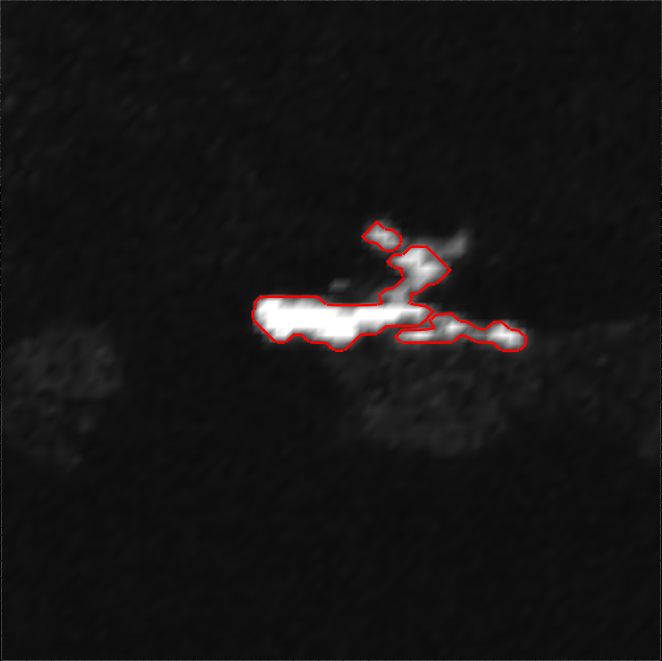
\includegraphics[scale=0.21]{pics/cropT2_otsu_tf.png}}
    \hspace{5px}
     \subfloat[cropT7] 
    {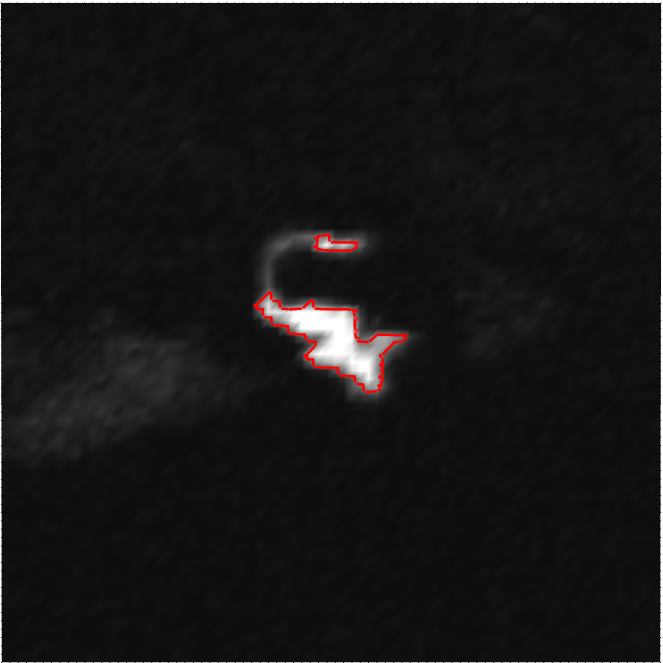
\includegraphics[scale=0.21]{pics/cropT7_otsu_tf.png}}
    \hspace{5px}
     \subfloat[cropT27] 
    {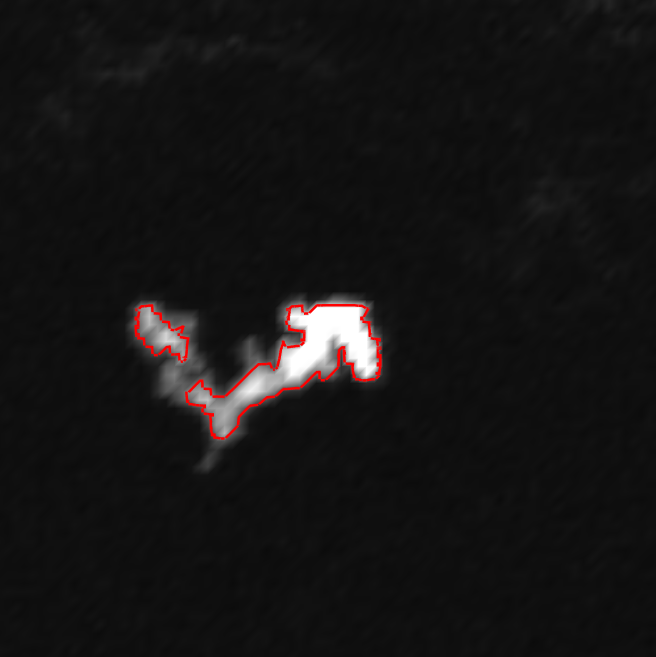
\includegraphics[scale=0.21]{pics/tst.png}}
    \hspace{5px}
     \subfloat[cropT45] 
    {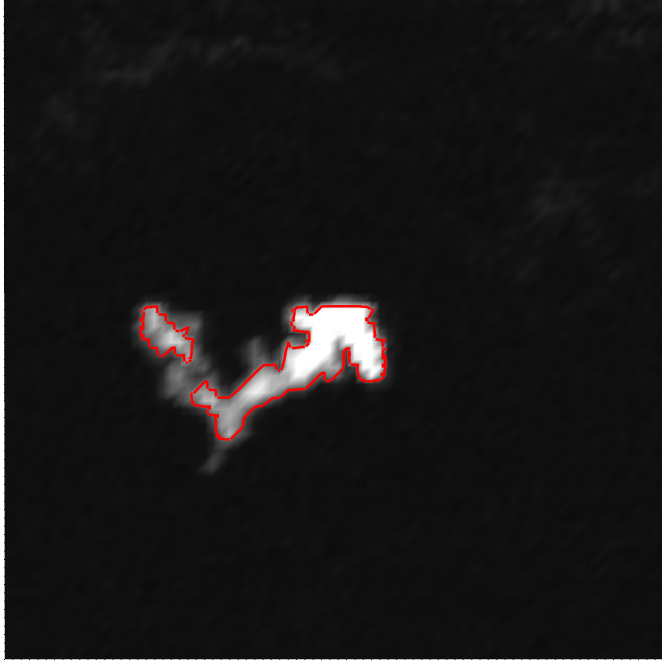
\includegraphics[scale=0.21]{pics/cropT45_otsu_tf1.png}}
    \caption{Výsledok segmentácie. Použitá Otsuho metóda a prahovacia funkcia.}
    \label{fig:otsu_tf}
\end{figure}

Ďalšou globálnou prahovacou metódou popísanoou v sekcii \ref{kapurM}, je metóda získavájúca prah pomocou maximálnej entropie zobrazená na obr. \ref{fig:kapur}. Môžeme si všimnúť, že prah tejto metódy bol určený o niečo vhodnejšie(vyšší) ako predošlá metóda, napríklad v prípade \ref{fig:kapur}c. Avšak pri tomto type prahovacej metódy sa môže stať,že makrofág bude obsahovať aj časti, ktoré pôvodne nemal.

\begin{figure}[H]  
\subfloat[cropT2]   
   {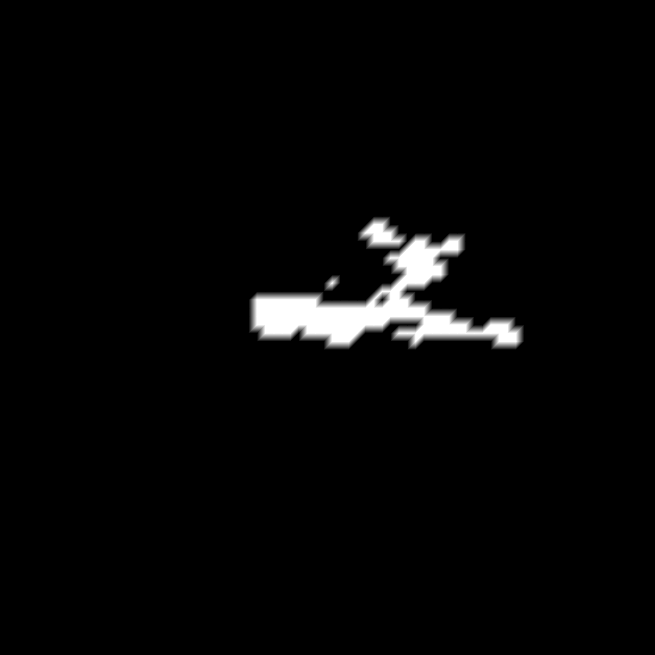
\includegraphics[scale=0.21]{pics/cropT2_kapur.png}}
    \hspace{5px}
    \subfloat[cropT7] 
   {
\includegraphics[scale=0.21]{pics/cropT7_kapur.png}}
    \hspace{5px}
     \subfloat[cropT27] 
    {
\includegraphics[scale=0.21]{pics/cropT27_kapur.png}}
    \hspace{5px}
    \subfloat[cropT45: prah = 73] 
   {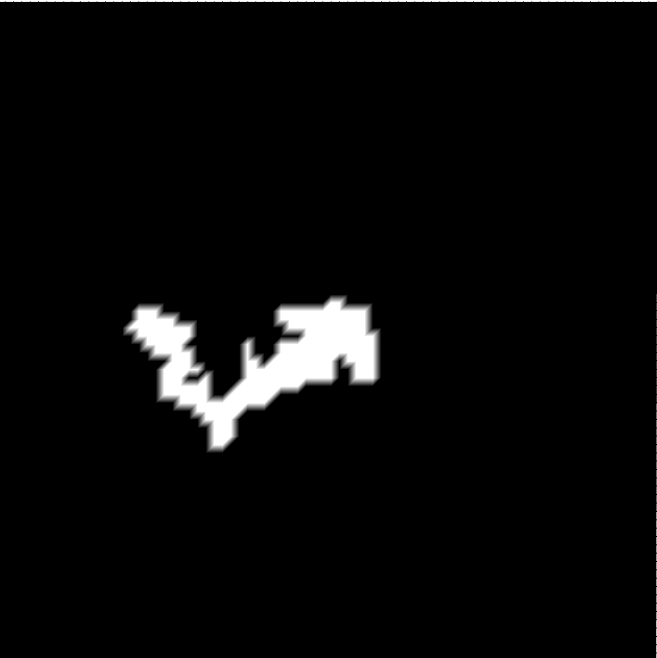
\includegraphics[scale=0.21]{pics/cropT45_kapur.png}}
    \caption{Prahovanie pomocou maximálnej entropie.}
    \label{fig:kapur}
\end{figure}

Výsledky segmentačnej metódy s počiatočnou podmienkou znamienkovej funkcie vzdialenosti obr. \ref{fig:kapur_sdf}.

%Vo výsledkoch \ref{fig:kapur_res} vidieť, že objekty obsahujú niektoré časti, ktoré sa na pôvodných dátach nenachádzajú a v niektorých prípadoch neobsahujú všetky časti. 

\begin{figure}[H]  
\subfloat[cropT2]   
   {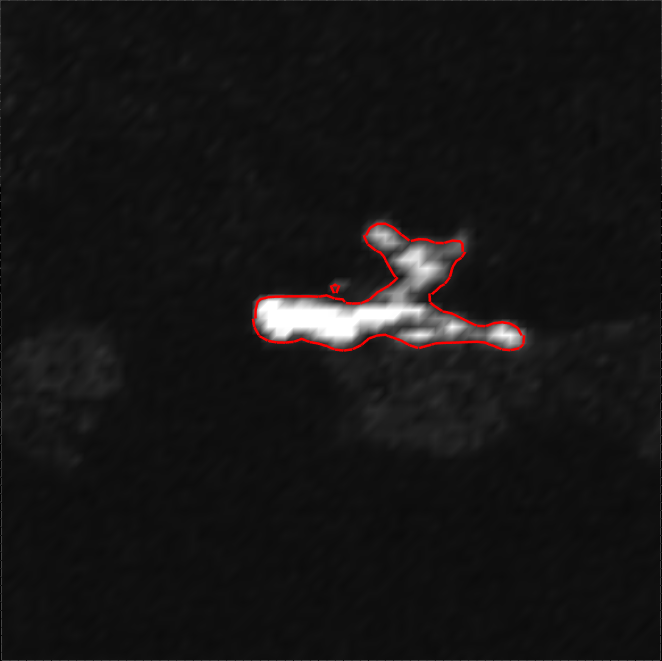
\includegraphics[scale=0.21]{pics/cropT2_kapur_sdf.png}}
    \hspace{5px}
    \subfloat[cropT7] 
   {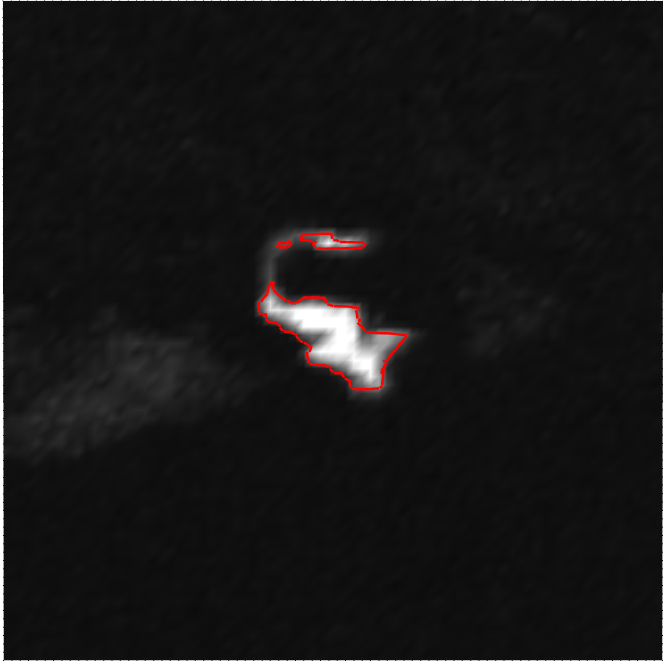
\includegraphics[scale=0.21]{pics/cropT7_kapur_sdf.png}}
    \hspace{5px}
     \subfloat[cropT27] 
    {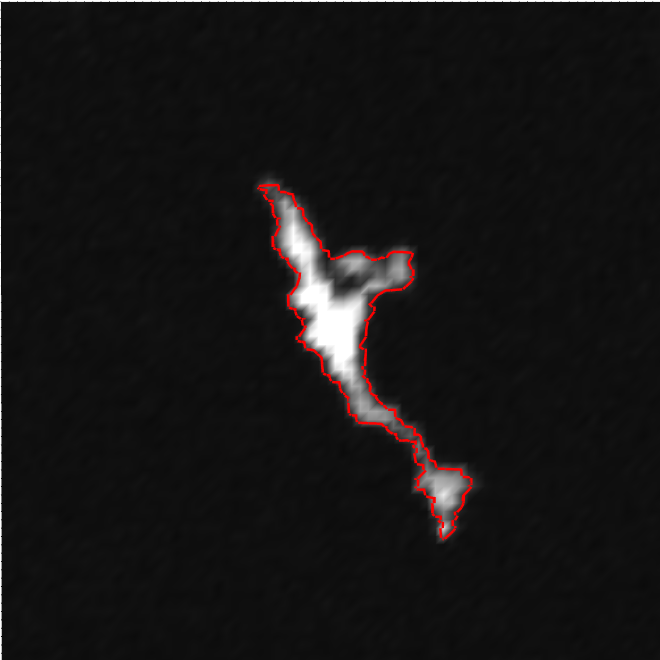
\includegraphics[scale=0.21]{pics/cropT27_kapur_sdf.png}}
    \hspace{5px}
    \subfloat[cropT45] 
   {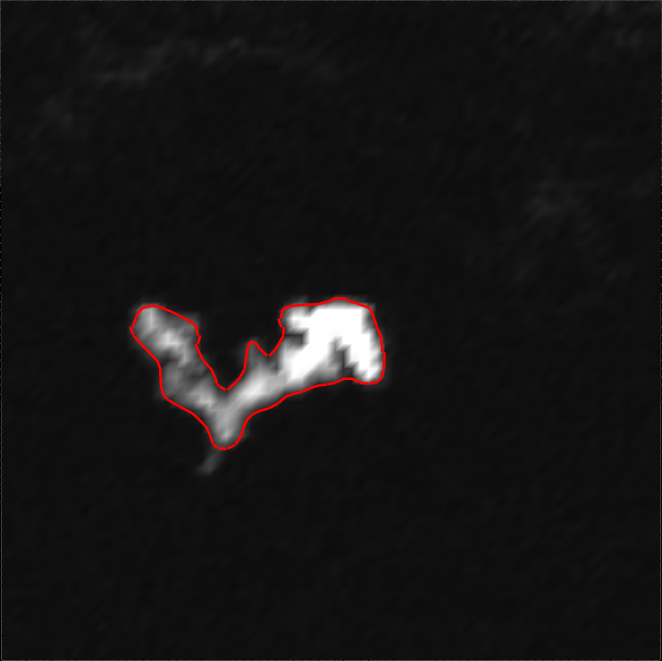
\includegraphics[scale=0.21]{pics/cropT45_kapur_sdf.png}}
    \caption{Výsledok segmentácie. Použité prahovanie pomocou maximálnej entropie a znamienková funkcia vzdialenosti.}
    \label{fig:kapur_sdf}
\end{figure}

Výsledky segmentačnej metódy s počiatočnou podmienkou prahovacej funkcie obr. \ref{fig:kapur_tf}.

\begin{figure}[H]  
\subfloat[cropT2]   
   {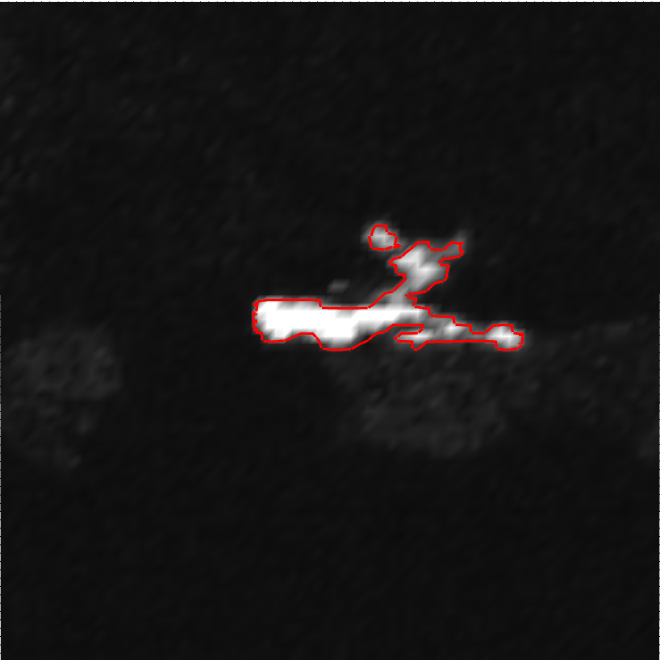
\includegraphics[scale=0.21]{pics/cropT2_kapur_tf.png}}
    \hspace{5px}
    \subfloat[cropT7] 
   {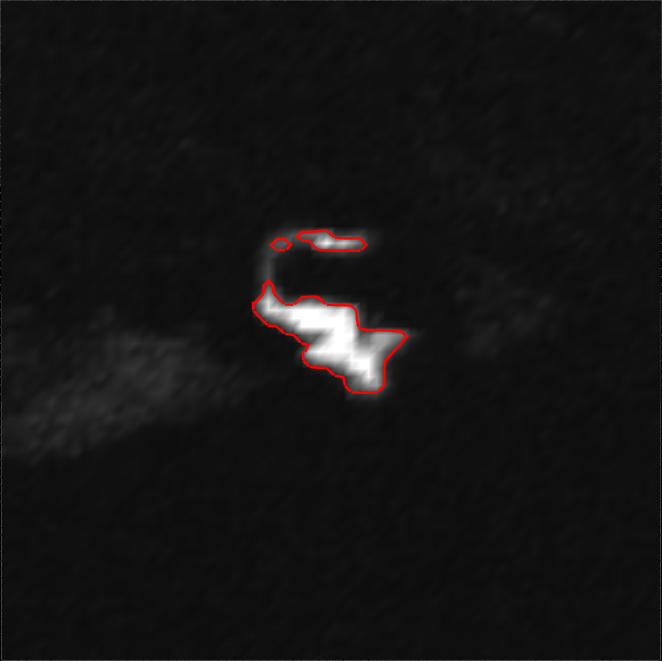
\includegraphics[scale=0.21]{pics/cropT7_kapur_tf.png}}
    \hspace{5px}
     \subfloat[cropT27] 
    {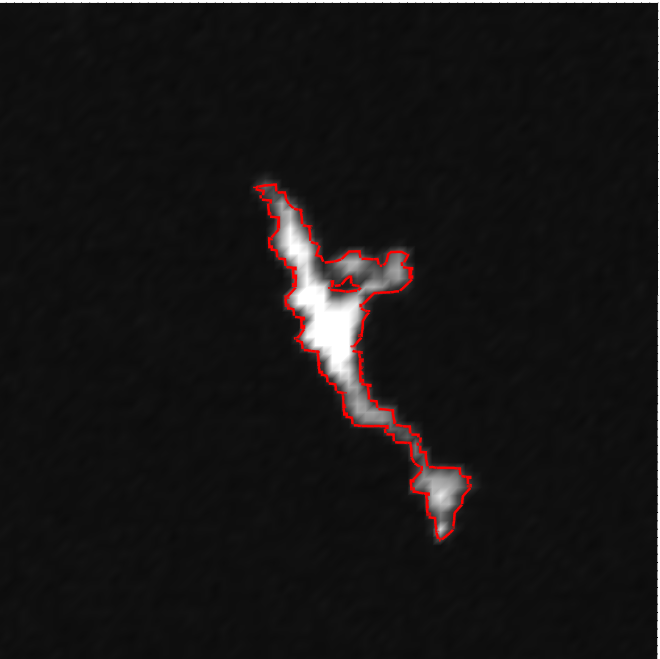
\includegraphics[scale=0.21]{pics/cropT27_kapur_tf.png}}
    \hspace{5px}
    \subfloat[cropT45] 
   {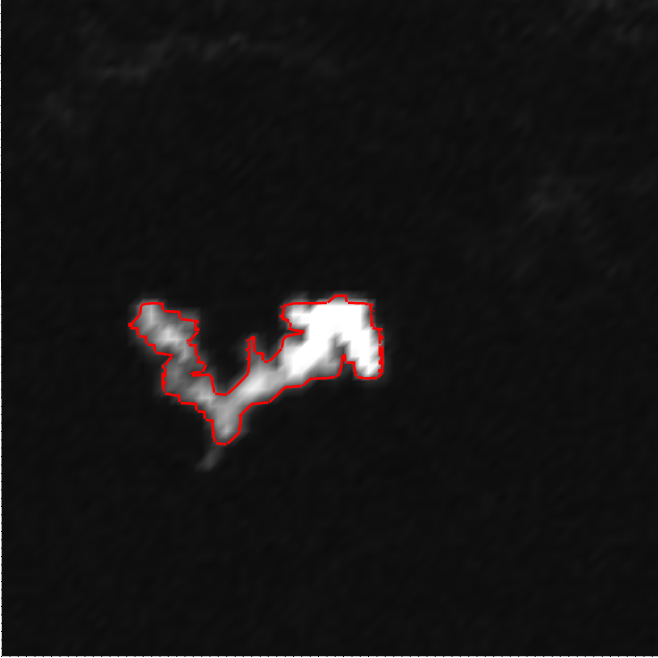
\includegraphics[scale=0.21]{pics/cropT45_kapur_tf.png}}
    \caption{Výsledok segmentácie. Použité prahovanie pomocou maximálnej entropie a prahovacia funkcia.}
    \label{fig:kapur_tf}
\end{figure}

Lepšie výsledky získane z aplikácii globálnych prahovacích metód na dáta získame pomocou nájdením prahu cez maximálnu entropiu a počiatočnej podmienky znamienkovej funkcie vzdialenosti.

V prípade lokálnych adaptívnych prahovacích metód je prah vyhodnotený pre každý pixel osobitne na nejakom fixne danom okolí, teda sme predpokladali, že výsledky týchto metód budú viac vyhovovať pri segmentácii makrofágov. Avšak tieto metódy závisia minimálne od veľkosti masky $m$, na ktorej sa počíta hodnota prahu pre zvolený pixel. A v niektorých prípadoch sa približne počíta priemer intenzít a smerodajná odchýlka pomocou jedného kroku rovnice vedenia, teda ďalším prametrom je veľkosť časového kroku $\sigma$. 

Prvou lokálnou adaptívnou metódou bola Niblackovej prahovacia metóda popísaná v sekcii \ref{niblack}.  S veľkosťou časového kroku $\sigma = 50.0,$ a veľkosťou masky $m = 3$, výsledky sú zobrazené na obr. \ref{fig:niblack}. 

\begin{figure}[H]  
\subfloat[cropT2]   
   {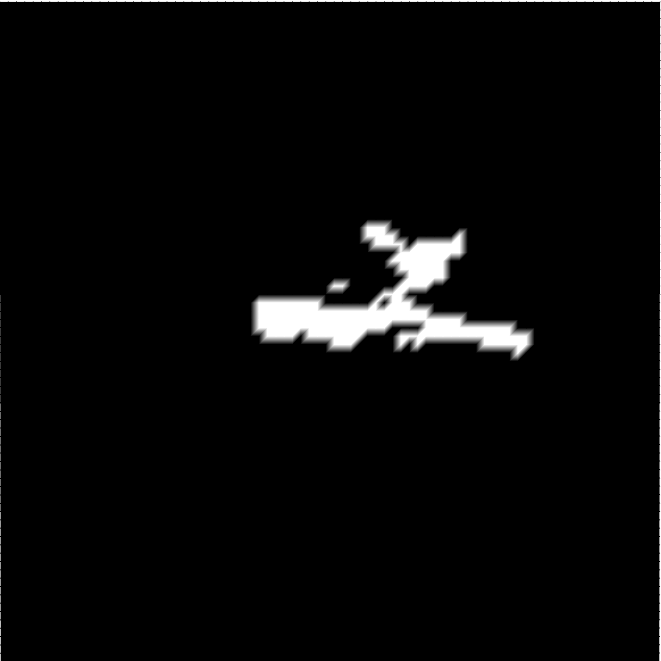
\includegraphics[scale=0.21]{pics/cropT2_niblack.png}}
    \hspace{5px}
    \subfloat[cropT7] 
   {
\includegraphics[scale=0.21]{pics/cropT7_niblack.png}}
    \hspace{5px}
     \subfloat[cropT27] 
    {\includegraphics[scale=0.21]{pics/cropT27_niblack.png}}
    \hspace{5px}
    \subfloat[cropT45] 
   {\includegraphics[scale=0.21]{pics/cropT45_niblack.png}}
    \caption{Niblackova segmentačná metóda.}
    \label{fig:niblack}
\end{figure}

Výsledky segmentačnej metódy s počiatočnou podmienkou znamienkovej funkcie vzdialenosti obr. \ref{fig:niblack_sdf}.

%Na obr. \ref{fig:niblack_sdf} sú zobrazené výsledky, kde boli na vstup ako okrajová podmienka uvažované dáta z Niblackovej prahovacej metódy.

\begin{figure}[H]  
\subfloat[cropT2]   
   {\includegraphics[scale=0.21]{pics/cropT2_niblack_sdf.png}}
    \hspace{5px}
    \subfloat[cropT7] 
   {\includegraphics[scale=0.21]{pics/cropT7_niblack_sdf.png}}
    \hspace{5px}
     \subfloat[cropT27] 
    {\includegraphics[scale=0.21]{pics/cropT27_niblack_sdf.png}}
    \hspace{5px}
    \subfloat[cropT45] 
   {\includegraphics[scale=0.21]{pics/cropT45_niblack_sdf.png}}
    \caption{Výsledok segmentácie. Použitá Niblacková metóda a znamienková funkcia vzdialenosti.}
    \label{fig:niblack_sdf}
\end{figure}

Výsledky segmentačnej metódy s počiatočnou podmienkou prahovacej funkcie obr. \ref{fig:niblack_tf}.

\begin{figure}[H]  
\subfloat[cropT2]   
   {\includegraphics[scale=0.21]{pics/cropT2_niblack_tf.png}}
    \hspace{5px}
    \subfloat[cropT7] 
   {\includegraphics[scale=0.21]{pics/cropT7_niblack_tf.png}}
    \hspace{5px}
     \subfloat[cropT27] 
    {\includegraphics[scale=0.21]{pics/cropT27_niblack_tf.png}}
    \hspace{5px}
    \subfloat[cropT45] 
   {\includegraphics[scale=0.21]{pics/cropT45_niblack_tf.png}}
    \caption{Výsledok segmentácie. Použitá Niblacková metóda a prahovacia funkcia.}
    \label{fig:niblack_tf}
\end{figure}

Bernsenova prahovacia funkcia popísaná v sekcii \ref{bernsenM}, pre veľkosť masky $m = 2$, je zobrazená na \ref{fig:bernsen}.

\begin{figure}[H]  
\subfloat[cropT2]   
   {\includegraphics[scale=0.21]{pics/cropT2_bernsen.png}}
    \hspace{5px}
    \subfloat[cropT7] 
   {\includegraphics[scale=0.21]{pics/cropT7_bernsen.png}}
    \hspace{5px}
     \subfloat[cropT27] 
    {\includegraphics[scale=0.21]{pics/cropT27_bernsen.png}}
    \hspace{5px}
    \subfloat[cropT45] 
   {\includegraphics[scale=0.21]{pics/cropT45_bernsen.png}}
    \caption{Bernsenova metóda.}
    \label{fig:bernsen}
\end{figure}

Výsledky segmentačnej metódy s počiatočnou podmienkou znamienkovej funkcie vzdialenosti obr. \ref{fig:bernsen_sdf}.

%Výsledky segmentačnej metódy, s kde na vstup sme brali Bernsenove prahovanie na obr. \ref{fig:bernsen_res}.

\begin{figure}[H]  
\subfloat[cropT2]   
   {\includegraphics[scale=0.21]{pics/cropT2_bernsen_sdf.png}}
    \hspace{5px}
    \subfloat[cropT7] 
   {\includegraphics[scale=0.21]{pics/cropT7_bernsen_sdf.png}}
    \hspace{5px}
     \subfloat[cropT27] 
    {\includegraphics[scale=0.21]{pics/cropT27_bernsen_sdf.png}}
    \hspace{5px}
    \subfloat[cropT45] 
   {\includegraphics[scale=0.21]{pics/cropT45_bernsen_sdf.png}}
    \caption{Výsledok segmentácie. Použitá Bernsenova metóda a znamienková funkcia vzdialenosti.}
    \label{fig:bernsen_sdf}
\end{figure}

Výsledky segmentačnej metódy s počiatočnou podmienkou prahovacej funkcie obr. \ref{fig:bernsen_tf}.

\begin{figure}[H]  
\subfloat[cropT2]   
   {\includegraphics[scale=0.21]{pics/cropT2_bernsen_tf.png}}
    \hspace{5px}
    \subfloat[cropT7] 
   {\includegraphics[scale=0.21]{pics/cropT7_bernsen_tf.png}}
    \hspace{5px}
     \subfloat[cropT27] 
    {\includegraphics[scale=0.21]{pics/cropT27_bernsen_tf.png}}
    \hspace{5px}
    \subfloat[cropT45] 
   {\includegraphics[scale=0.21]{pics/cropT45_bernsen_tf.png}}
    \caption{Výsledok segmentácie. Použitá Bernsenova metóda a prahovacia funkcia.}
    \label{fig:bernsen_tf}
\end{figure}

Sauvolova prahovacia metóda bola upravená z Niblackovej a používa sa primárne primárne používa na prahovanie textových obrazových dát ale keďže makrofágy sú malé a majú nepravidelné tvary, tak sme predpokladali, že aj v našom prípade by mohla dávať uspokojivé výsledky. Na obr. \ref{fig:sauvola} s parametrami $\sigma = 50.0$ a $m = 3$.

\begin{figure}[H]  
\subfloat[cropT2]   
   {\includegraphics[scale=0.21]{pics/cropT2_sauvola.png}}
    \hspace{5px}
    \subfloat[cropT7] 
   {\includegraphics[scale=0.21]{pics/cropT7_sauvola.png}}
    \hspace{5px}
     \subfloat[cropT27] 
    {\includegraphics[scale=0.21]{pics/cropT27_sauvola.png}}
    \hspace{5px}
    \subfloat[cropT45] 
   {\includegraphics[scale=0.21]{pics/cropT45_sauvola.png}}
    \caption{Sauvolova metóda.}
    \label{fig:sauvola}
\end{figure}

Výsledky segmentačnej metódy s počiatočnou podmienkou znamienkovej funkcie vzdialenosti obr. \ref{fig:sauvola_sdf}.

\begin{figure}[H]  
\subfloat[cropT2]   
   {\includegraphics[scale=0.21]{pics/cropT2_sauvola_sdf.png}}
    \hspace{5px}
    \subfloat[cropT7] 
   {\includegraphics[scale=0.21]{pics/cropT7_sauvola_sdf.png}}
    \hspace{5px}
     \subfloat[cropT27] 
    {\includegraphics[scale=0.21]{pics/cropT27_sauvola_sdf.png}}
    \hspace{5px}
    \subfloat[cropT45] 
   {\includegraphics[scale=0.21]{pics/cropT45_sauvola_sdf.png}}
    \caption{Výsledok segmentácie. Použitá Sauvolova metóda a znamienková funkcia vzdialenosti.}
    \label{fig:sauvola_sdf}
\end{figure}

Výsledky segmentačnej metódy s počiatočnou podmienkou prahovacej funkcie obr. \ref{fig:sauvola_tf}.

\begin{figure}[H]  
\subfloat[cropT2]   
   {\includegraphics[scale=0.21]{pics/cropT2_sauvola_tf.png}}
    \hspace{5px}
    \subfloat[cropT7] 
   {\includegraphics[scale=0.21]{pics/cropT7_sauvola_tf.png}}
    \hspace{5px}
     \subfloat[cropT27] 
    {\includegraphics[scale=0.21]{pics/cropT27_sauvola_tf.png}}
    \hspace{5px}
    \subfloat[cropT45] 
   {\includegraphics[scale=0.21]{pics/cropT45_sauvola_tf.png}}
    \caption{Výsledok segmentácie. Použitá Sauvolova metóda a prahovacia funkcia.}
    \label{fig:sauvola_tf}
\end{figure}

Poslednými dvomi lokálnymi adaptívnymi metódami sú hybridné metódy používajúce princípy z predchádzajúcich metód. 
 
Prvá hybridná metóda vznikla kombináciou Bernsenovej a Nicblackovej metódy na obr. \ref{fig:hybrid1}  sú zobrazené výsledky s parametrami $\sigma = 50.0$ a $m = 3$.

\begin{figure}[H]  
\subfloat[cropT2]   
   {\includegraphics[scale=0.21]{pics/cropT2_hybrid_nb.png}}
    \hspace{5px}
    \subfloat[cropT7] 
   {\includegraphics[scale=0.21]{pics/cropT7_hybrid_nb.png}}
    \hspace{5px}
     \subfloat[cropT27] 
    {\includegraphics[scale=0.21]{pics/cropT27_hybrid_nb.png}}
    \hspace{5px}
    \subfloat[cropT45] 
   {\includegraphics[scale=0.21]{pics/cropT45_hybrid_nb.png}}
    \caption{Hybridná Bernsenova a Niblackova metóda.}
    \label{fig:hybrid1}
\end{figure}

Výsledky segmentačnej metódy s počiatočnou podmienkou znamienkovej funkcie vzdialenosti obr. \ref{fig:hybrid1_sdf}.

\begin{figure}[H]  
\subfloat[cropT2]   
   {\includegraphics[scale=0.21]{pics/cropT2_hybrid_nb_sdf.png}}
    \hspace{5px}
    \subfloat[cropT7] 
   {\includegraphics[scale=0.21]{pics/cropT7_hybrid_nb_sdf.png}}
    \hspace{5px}
     \subfloat[cropT27] 
    {\includegraphics[scale=0.21]{pics/cropT27_hybrid_nb_sdf.png}}
    \hspace{5px}
    \subfloat[cropT45] 
   {\includegraphics[scale=0.21]{pics/cropT45_hybrid_nb_sdf.png}}
    \caption{Výsledok segmentácie. Použitá prvá hybridná prahovacia metóda a znamienková funkcia vzdialenosti.}
    \label{fig:hybrid1_sdf}
\end{figure}

Výsledky segmentačnej metódy s počiatočnou podmienkou prahovacej funkcie obr. \ref{fig:hybrid1_tf}.

\begin{figure}[H]  
\subfloat[cropT2]   
   {\includegraphics[scale=0.21]{pics/cropT2_hybrid_nb_tf.png}}
    \hspace{5px}
    \subfloat[cropT7] 
   {\includegraphics[scale=0.21]{pics/cropT7_hybrid_nb_tf.png}}
    \hspace{5px}
     \subfloat[cropT27] 
    {\includegraphics[scale=0.21]{pics/cropT27_hybrid_nb_tf.png}}
    \hspace{5px}
    \subfloat[cropT45] 
   {\includegraphics[scale=0.21]{pics/cropT45_hybrid_nb_tf.png}}
    \caption{Výsledok segmentácie. Použitá prvá hybridná metóda a prahovacia funkcia.}
    \label{fig:hybrid1_tf}
\end{figure}

Druhá hybridná metóda vznikla kombináciou Bernsenovej a Sauvolovej metódy na obr. \ref{fig:hybrid2}  sú zobrazené výsledky s parametrami $\sigma = 50.0$ a $m = 3$.

\begin{figure}[H]  
\subfloat[cropT2]   
   {\includegraphics[scale=0.21]{pics/cropT2_hybrid_sb.png}}
    \hspace{5px}
    \subfloat[cropT7] 
   {\includegraphics[scale=0.21]{pics/cropT7_hybrid_sb.png}}
    \hspace{5px}
     \subfloat[cropT27] 
    {\includegraphics[scale=0.21]{pics/cropT27_hybrid_sb.png}}
    \hspace{5px}
    \subfloat[cropT45] 
   {\includegraphics[scale=0.21]{pics/cropT45_hybrid_sb.png}}
    \caption{Hybridná Bernsenova a Sauvolova metóda.}
    \label{fig:hybrid2}
\end{figure}

Výsledky segmentačnej metódy s počiatočnou podmienkou znamienkovej funkcie vzdialenosti obr. \ref{fig:hybrid2_sdf}.

\begin{figure}[H]  
\subfloat[cropT2]   
   {\includegraphics[scale=0.21]{pics/cropT2_hybrid_sb_sdf.png}}
    \hspace{5px}
    \subfloat[cropT7] 
   {\includegraphics[scale=0.21]{pics/cropT7_hybrid_sb_sdf.png}}
    \hspace{5px}
     \subfloat[cropT27] 
    {\includegraphics[scale=0.21]{pics/cropT27_hybrid_sb_sdf.png}}
    \hspace{5px}
    \subfloat[cropT45] 
   {\includegraphics[scale=0.21]{pics/cropT45_hybrid_sb_sdf.png}}
    \caption{Výsledok segmentácie. Použitá druhá hybridná prahovacia metóda a znamienková funkcia vzdialenosti.}
    \label{fig:hybrid2_sdf}
\end{figure}

Výsledky segmentačnej metódy s počiatočnou podmienkou prahovacej funkcie obr. \ref{fig:hybrid2_tf}.

\begin{figure}[H]  
\subfloat[cropT2]   
   {\includegraphics[scale=0.21]{pics/cropT2_hybrid_sb_tf.png}}
    \hspace{5px}
    \subfloat[cropT7] 
   {\includegraphics[scale=0.21]{pics/cropT7_hybrid_sb_tf.png}}
    \hspace{5px}
     \subfloat[cropT27] 
    {\includegraphics[scale=0.21]{pics/cropT27_hybrid_sb_tf.png}}
    \hspace{5px}
    \subfloat[cropT45] 
   {\includegraphics[scale=0.21]{pics/cropT45_hybrid_sb_tf.png}}
    \caption{Výsledok segmentácie. Použitá druhá hybridná metóda a prahovacia funkcia.}
    \label{fig:hybrid2_tf}
\end{figure}

%Z výsledkov na obrázkoch \ref{fig:otsu_res}, \ref{fig:kapur_res}, \ref{fig:niblack_res} a \ref{fig:bernsen_res}  vidieť, že vhodnejšími prahovacími metódami vstupujúcimi do segmentácie ako okrajová podmienka sú lokálne adaptívne prahovacie metódy. A Niblackova prahovacia metóda obr. obr \ref{fig:niblack} najlepšie popisuje skutočný tvar makrofágu.

Zo zobrazených výsledkov si môžeme všimnúť že výrazne lepšie výsledky získame pri použití niektorých z lokálnych adaptívnych prahovacích metód, ale napr. pri Sauvolovej prahovaciej funkcii je zachytený aj šum patriaci pozadiu. Najlepšie výsledky sme dostali použitím počiatočnej podmienky z hybridnej Bernsenovej a Niblackovej prahovej funkcie. 

\newpage
\section{Záver}

%Cieľom tejto práce, bolo nájsť 

\newpage
\begin{thebibliography}{50}

\bibitem{vtk} 
\textbf{VTK dokumentácia}:
\url{https://vtk.org/documentation/},

\bibitem{qt} 
\textbf{Qt dokumentácia}:
\url{https://doc.qt.io/},

\bibitem{sora} 
Seol Ah Park, Tamara Sipka, Zuzana Krivá, Martin Ambroz, Michal Kollar, Balazs Kosa, Mai Nguyen-Chi, Georges Lutfalla, Karol Mikula, \textbf{Macrophage image segmentation by Thresholding and subjective surface Method}: \\ 
\url{https://www.researchgate.net/publication/337755994_Macrophage_image_segmentation_by_Thresholding_and_subjective_surface_Method},

\bibitem{skripta} 
Zuzana Krivá, Karol Mikula, Oľqa Stašová, \textbf{Spracovanie obrazu vybrané kapitoly z prednášok}, 
%\url{http://money.cnn.com/2018/03/19/technology/facebook-data-scandal-explainer/index.html}.

\bibitem{skripta1} 
Wilhelm Burger, \textbf{Principles of Digital Image Processing: Core Algorithms},
%: \\ \url{https://panopticlick.eff.org/about#browser-fingerprinting}.

\bibitem{hybridNBaBren} 
Anna Korzynska, Lukasz Roszkowiak,Carlos Lopez, Ramon Bosch, Lukasz Witkowski1,  Marylene Lejeune \textbf{Validation of various adaptive thresholdmethods of segmentation applied to follicularlymphoma digital images stained with3,3’-Diaminobenzidine$\&$Haematoxylin}: 
\url{https://www.ncbi.nlm.nih.gov/pmc/articles/PMC3656801/},

\bibitem{otsu} 
Nobuyuki Otsu, \textbf{A Threshold Selection Method from Gray-Level Histograms}, 



\end{thebibliography}

\end{document}